\documentclass{thesisclass}
% Based on thesisclass.cls of Timo Rohrberg, 2009
% ----------------------------------------------------------------
% Thesis - Main document
% ----------------------------------------------------------------


%% -------------------------------
%% |  Information for PDF file   |
%% -------------------------------
\hypersetup{
 pdfauthor={Manuel Schweigert},
 pdftitle={Distrubuted Node Coloring Algorithms for Directed Graphs},
 pdfsubject={Bachelor Thesis},
 pdfkeywords={Distrubuted, Node, Coloring, Algorithms, Directed Graphs, Manuel Schweigert, Bachelor, Thesis}
}


%% ---------------------------------
%% | Information about the thesis  |
%% ---------------------------------

\newcommand{\myname}{Manuel Schweigert}
\newcommand{\mytitle}{Distributed Node Coloring Algorithms for Directed Graphs}
\newcommand{\myinstitute}{Institute of Theoretical Computer Science}

\newcommand{\reviewerone}{Prof. Dr. Dorothea Wagner}
\newcommand{\reviewertwo}{Prof. Dr. Peter Sanders}
\newcommand{\advisor}{Dipl. Inform. Fabian Fuchs}
\newcommand{\advisortwo}{Dipl. Inform. Roman Putkin}

\newcommand{\timestart}{13th of January 2014}
\newcommand{\timeend}{12th of May 2014}


%% ---------------------------------
%% | Commands                      |
%% ---------------------------------

\newtheorem{definition}{Definition} \numberwithin{definition}{chapter}
\newtheorem{theorem}[definition]{Theorem}
\newtheorem{lemma}[definition]{Lemma}
\newtheorem{corollary}[definition]{Corollary}
\newtheorem{conjecture}[definition]{Conjecture}

\newcommand{\defines}{\mathrel{\mathop{\raisebox{1pt}{\scriptsize$:=$}}}}

\newenvironment{myindent}[1]%
{\begin{list}{}%
         {\setlength{\leftmargin}{#1}}%
         \item[]%
}
{\end{list}}


%% --------------------------------
%% | Settings for word separation |
%% --------------------------------
% Help for separation:
% In german package the following hints are additionally available:
% "- = Additional separation
% "| = Suppress ligation and possible separation (e.g. Schaf"|fell)
% "~ = Hyphenation without separation (e.g. bergauf und "~ab)
% "= = Hyphenation with separation before and after
% "" = Separation without a hyphenation (e.g. und/""oder)

% Describe separation hints here:
\hyphenation{
% Pro-to-koll-in-stan-zen
% Ma-na-ge-ment  Netz-werk-ele-men-ten
% Netz-werk Netz-werk-re-ser-vie-rung
% Netz-werk-adap-ter Fein-ju-stier-ung
% Da-ten-strom-spe-zi-fi-ka-tion Pa-ket-rumpf
% Kon-troll-in-stanz
}


%% ------------------------
%% |    Including files   |
%% ------------------------
% Only files listed here will be included!
% Userful command for partially translating the document (for bug-fixing e.g.)
\includeonly{
titlepage,
introduction,
preliminaries,
content,
conclusion,
appendix
}

\usepackage{indentfirst}
\usepackage{subcaption}
\usepackage{tabularx}
\DeclareCaptionSubType * {figure}
\renewcommand\thesubfigure{\thefigure\alph{subfigure}}
\setlength{\parindent}{15pt}

\DeclareMathOperator{\dist}{dist}
\DeclareMathOperator{\range}{range}


%%%%%%%%%%%%%%%%%%%%%%%%%%%%%%%%%
%% Here, main documents begins %%
%%%%%%%%%%%%%%%%%%%%%%%%%%%%%%%%%
\begin{document}

% Remove the following line for German text
\selectlanguage{english}

\frontmatter
\pagenumbering{roman}
%% titlepage.tex
%%

% coordinates for the bg shape on the titlepage
\newcommand{\diameter}{7}
\newcommand{\xone}{-15}
\newcommand{\xtwo}{160}
\newcommand{\yone}{15}
\newcommand{\ytwo}{-253}

\begin{titlepage}
% bg shape
\begin{tikzpicture}[overlay]
\draw[color=gray]  
 		 (\xone mm, \yone mm)
  -- (\xtwo mm, \yone mm)
 arc (90:0:\diameter mm) 
  -- (\xtwo mm + \diameter mm , \ytwo mm) 
	-- (\xone mm + \diameter mm , \ytwo mm)
 arc (270:180:\diameter mm)
	-- (\xone mm, \yone mm);
\end{tikzpicture}
	\begin{textblock}{10}[0,0](4,2.5)
		
\includegraphics[width=.3\textwidth]{logos/KITLogo.pdf}
	\end{textblock}
        \begin{textblock}{10}[0,0](14.5,2.45)
		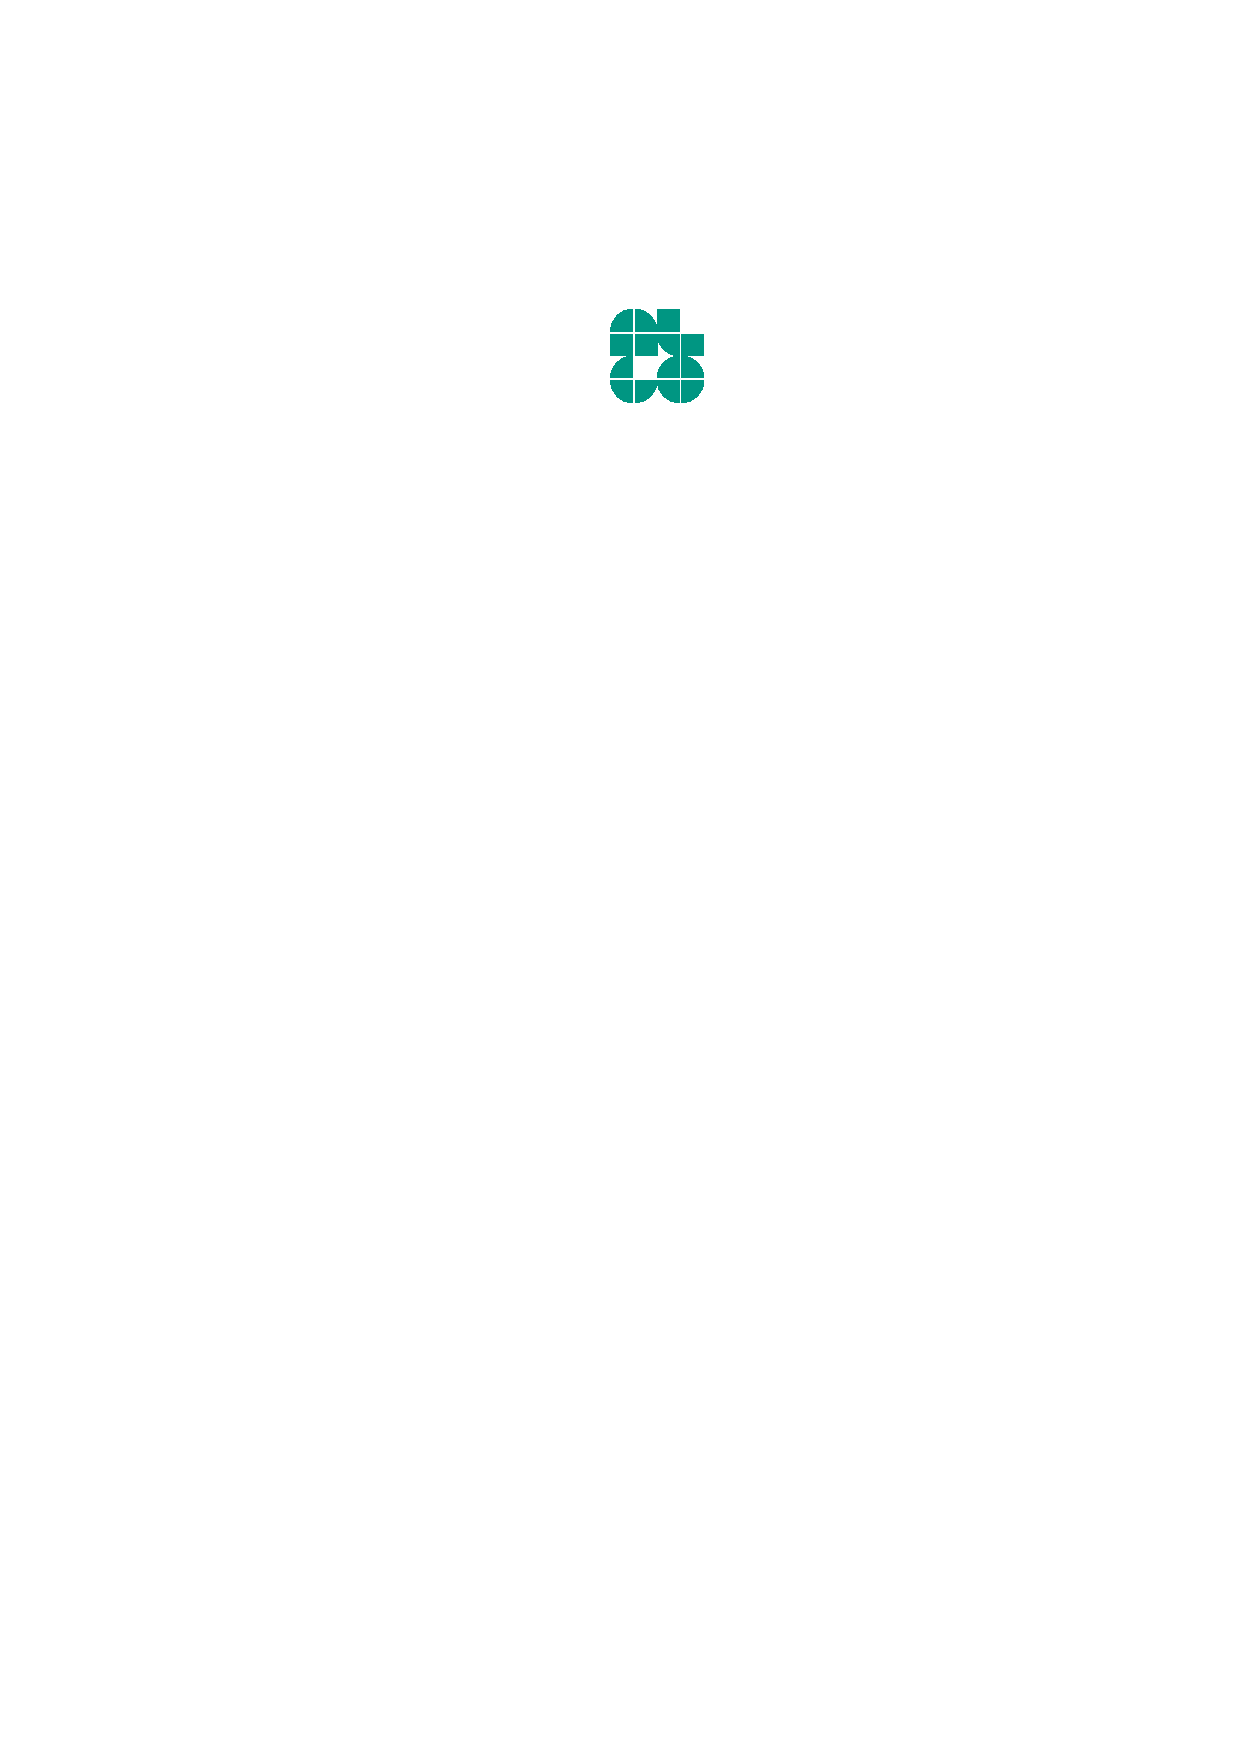
\includegraphics[width=.15\textwidth]{logos/algoLogo.pdf}
	\end{textblock}
	\changefont{phv}{m}{n}	% helvetica	
	\vspace*{3.75cm}
	\begin{center}
		\Huge{\mytitle}
		\vspace*{2.25cm}\\
		\Large{
			\iflanguage{english}{Bachelor Thesis of}			
												  {Diplomarbeit\\von}
		}\\
		\vspace*{1cm}
		\huge{\myname}\\
		\vspace*{1cm}
		\Large{
			\iflanguage{english}{At the Department of Informatics}			
													{An der Fakult\"at f\"ur Informatik}
			\\
			\myinstitute
		}
	\end{center}
	\vspace*{1cm}
\Large{
\begin{center}
\begin{tabular}[ht]{l c l}
  % Gutachter sind die Professoren, die die Arbeit bewerten. 
  \iflanguage{english}{Reviewers}{Erstgutachter}: & \hfill & \reviewerone\\
  \iflanguage{english}{}{Zweitgutachter:} & \hfill & \reviewertwo\\
  \iflanguage{english}{Advisors}{Betreuende Mitarbeiter}: & \hfill & \advisor\\
  \iflanguage{english}{}{} & \hfill & \advisortwo\\
  % Der zweite betreuende Mitarbeiter kann weggelassen werden. 
\end{tabular}
\end{center}
}


\vspace{2cm}
\begin{center}
\large{\iflanguage{english}{Time Period}{Bearbeitungszeit}: \ \timestart{} \ -- \ \timeend}
\end{center}


\begin{textblock}{10}[0,0](4,16.8)
\tiny{ 
	\iflanguage{english}
		{KIT -- University of the State of Baden-Wuerttemberg and National Laboratory of the Helmholtz Association}
		{KIT -- Universit�t des Landes Baden-W�rttemberg und nationales Forschungszentrum der Helmholtz-Gesellschaft}
}
\end{textblock}

\begin{textblock}{10}[0,0](14,16.75)
\large{
	\textbf{www.kit.edu} 
}
\end{textblock}

\end{titlepage}

\blankpage

%% -------------------------------
%% |   Statement of Authorship   |
%% -------------------------------

\thispagestyle{plain}

\vspace*{\fill}

\centerline{\bf Statement of Authorship}

\vspace{0.25cm}

I hereby declare that this document has been composed by myself and describes my own work, unless otherwise acknowledged in the text.

\vspace{2.5cm}

\hspace{0.25cm} Karlsruhe, \today

\vspace{2cm}

\blankpage

%% -------------------
%% |   Abstract      |
%% -------------------

\thispagestyle{plain}

\begin{addmargin}{0.5cm}

\centerline{\bf Abstract}

Distributed node coloring algorithms are the heart of creating efficient, collision free communication schemes in ad hoc wireless communication networks such as sensor networks. As such, there is great practical importance in understanding these algorithms and in creating models which are as close to reality as possible, such as the Signal to Interference and Noise Ratio (SINR) communication model.

In this thesis, we analyze the implications of different transmission ranges of nodes on coloring algorithms, resulting in an underlying directed graph problem. We show that a chain of unidirectional communication links will have an effect on the run times of algorithms, but otherwise will not prohibit a valid coloring to be computed.

We present randomized algorithms roughly based on Luby's algorithm \cite{luby1986simple}, which produce $\Delta+1$-colorings in $O(\Delta + l \log n)$ and $2\Delta+1$-colorings in $O(l \log n)$ broadcast rounds. We also present observations from our simulations that $l$ depends on the deviation in transmission ranges.

\vskip 2cm

\centerline{\normalfont \bfseries Deutsche Zusammenfassung}

\noindent Algorithmen zur Knotenfärbung sind das Herzstück effizienter, kollisionsfreier Kommunikationsschemata in drahtlosen Ad-hoc-Netzwerken, wie sie beispielsweise in Sensornetzwerken vorkommen. Daher gibt es ein großes, praktisches Interesse daran, diese Algorithmen zu verstehen und Modelle zu entwerfen, die realitätsnahe Ergebnisse liefern können, wie zum Beispiel das Signal to Interference and Noise Ratio (SINR) Modell.

\noindent In dieser Arbeit widmen wir uns dem Entwurf und der Analyse von Algorithmen, welche auf der Annahme basieren, dass Knoten im SINR Modell (aufgrund verschiedener Sendeleistungen) verschieden große Übertragungsreichweiten haben können. Dies impliziert ein Graphenmodell, welches unidirektionale Kanten erlaubt, da Knoten nicht unbedingt genug Reichweite zum Antworten haben.

\noindent Wir stellen unter anderem randomisierte Algorithmen vor, die in einer Laufzeit von $O(\Delta + l \log n)$ bzw. $O(l \log n)$ eine $\Delta+1$ bzw. eine $2\Delta+1$ Färbung mit hoher Wahrscheinlichkeit erstellen. Hierbei ist $\Delta$ der maximale Knoten-Eingangsgrad, $n$ die Knotenanzahl und $l$ die Länge der längsten unidirektionalen Kette im Graphen. Wir stellen schließlich eine experimentelle Studie zur Länge von $l$ an und kommen zu dem Ergebnis, dass $l$ von der Standardabweichung der Übertragungsreichweiten der Knoten im Graphen abhängt.

\end{addmargin}

\blankpage

%% -------------------
%% |   Directories   |
%% -------------------

\tableofcontents
\blankpage

%% -----------------
%% |   Main part   |
%% -----------------

\mainmatter
\pagenumbering{arabic}
%% introduction.tex
%%

%% ==============================
\chapter{Introduction}
\label{ch:introduction}
%% ==============================

Ad hoc wireless radio networks became more prevalent recently and will continue to grow, as mobile devices, vehicles, drones and sensors are on the rise both in the market and in research. However, when these devices get deployed, they lack any global knowledge of their environment and might not have any reliable infrastructure to coordinate their actual tasks efficiently.

To enable efficient communication between these nodes, and with that to enable them to make use of well-studied algorithms for distributed settings, a network organization protocol must be established first. Such a protocol can be established in a fully distributed environment on a single radio frequency band by using a Time Division Multiple Access (TDMA) scheme to create a Medium Access Control (MAC) layer on that band. By assigning each node timeslots in a way, such that interference between simultaneous senders is low, such a protocol would avoid message-collisions and enable efficient communication.

Creating a TDMA scheme in a network without any initial structure is therefore of great practical importance and a lot of research has been done on this subject in the recent past. The theoretical problem of coloring neighboring nodes in a graph with different colors is a closely related problem which has therefore seen a lot of attention recently. While theoretically, a simple node coloring can be translated into a TDMA scheme by assigning each node a timeslot according to its color, this does not guarantee a collision-free structure. It is generally known that a distance-2 coloring is sufficient for that (e.g. \cite{ramanathan1993scheduling}), meaning that for a node $v$, and each pair of distinct neighbours $u$ and $w$, their colors must not match respectively.

However, it has been shown that in practice, a simple node coloring is already too restrictive when translated to a TDMA scheme \cite{moscibroda2006protocol}. This means that for most purposes, efficiently calculating a valid node coloring in an unstructured network is the key to enabling any further complexity.

The chosen model of the graph structure and communication play huge part in the distributed complexity of an algorithm calculating such a coloring. While early works have made assumptions that enabled algorithms to perform in good asymptotic complexities, the focus shifts more and more towards models which are closer to reality and therefore give better predictions and boundaries for practical solutions.

One model which has seen a lot of attention recently is the Signal to Interference and Noise Ratio (SINR) model. While this model only accounts for the environment by a static noise constant, it takes into account the interference caused by all sending nodes in a network at a given time and by comparing the signal strength of the senders signal to the sum of interfering signals, the model determines whether a message-delivery was successful or not.

Theoretically, every node in this model may have a different transmission power, yet most works so far have artificially restricted transmission powers to a uniform value, because uniform transmission ranges correspond to unit disk graphs, which are well understood and behave nicely. As this defeats the purpose of having a model closer to reality, recent works have taken steps towards removing these restraints. For example, to allow arbitrary transmission power in the SINR model, only few changes in known local broadcasting algorithms are necessary \cite{DBLP:journals/corr/FuchsW14}. This results in a disk graph model, which suggests that bidirectional communication is not always possible.

We therefore analyze what is necessary to compute a coloring in a directed graph using the CONGEST model, abstracting away the local broadcast which can be done in $O(\Gamma^2 \Delta \log n)$ timeslots \cite{DBLP:journals/corr/FuchsW14}. We discuss the graph and communication models in more detail in Sections \ref{section:comm} and \ref{section:graph}.

\section{Related Work}

Graph coloring is one of the oldest theoretical problems of computer science (\cite{birkhoff1912determinant}, \cite{whitney1931coloring}), however the distributed aspect has only recently seen a lot of attention. Early on, Cole and Vishkin proposed a deterministic algorithm which would 3-color a cycle ($\Delta+1$) in a run time of $O(\log^* n)$ \cite{cole1986deterministic}. Many authors worked to improve and further analyze this algorithm and it has finally been shown by Goldberg and Plotkin to work in any bounded degree graphs with the same run time \cite{goldberg1987parallel}. 

This run time is asymptotically tight as a lower bound of $\Omega(\log^* n)$ for the distributed graph coloring was shown by Linial \cite{linial1992locality}. This bound is even true for randomized algorithms, such as the ones considered in this thesis.

Another very popular $\Delta+1$ algorithm which was first introduced by Schneider and Wattenhofer is based on the maximal independent set (MIS) problem and creates a coloring in $O(\log^* n)$ for growth bounded graphs by using an MIS algorithm together with a color reduction technique \cite{schneider2008log}. 

Motivated by the challenges of unstructured radio networks, Moscibroda and Wattenhofer adapted that algorithm to accomodate for a lack of collision detection and asynchronous wake up times and created an algorithm capable of operating in a more realistic model. It produced an $O(\Delta)$ coloring in $O(\log n)$ time, while minimizing the number of colors locally. Derbel and Talbi improved this algorithm further by adapting it to the Signal to Interference and Noise Ratio (SINR) physical model, which is another step into the direction of realism \cite{dt-dncsi-10}. Their algorithm also produces an $O(\Delta)$ coloring while needing $O(\Delta \log n)$ time slots, which is impressive considering that a simple round of conventional message passing in that model needs the same amount of time \cite{goussevskaia2008local}. 

Research has also been done on defective coloring, which means algorithms produce colorings which are invalid up to a certain degree, as it was shown that a normal coloring may already be too restrictive for an effective TDMA scheme \cite{moscibroda2006protocol}. These defective coloring algorithms and current randomized algorithms have recently been gathered in a monograph by Barenboim and Elkin \cite{be-dcg-13}. 

Graph colorings in networks with arbitrary transmission power have so far only been looked at in \cite{DBLP:journals/corr/FuchsW14} with a suggested algorithm which produces $O(\Gamma^2 \Delta)$-colorings in $O((\Delta+l)\Gamma^6 \Delta \log n)$ timeslots in the SINR model, which corresponds to $O(\Delta)$ colors with $O(\Delta + l \log n)$ rounds in the CONGEST model. In this work we improve on the run time and the number of colors by utilizing randomized algorithms.

\section{Contributions}

In this thesis we take a popular class of simple randomized algorithms and look into what changes when the underlying graph model becomes less restricted. For this purpose, we first analyze this graph model and the challenges it represents, which are unidirectional communication links.

To bypass this problem, we take a simple algorithm to compute a $2\Delta$ coloring and add an initialization to it, so that a node knows if it is dominated, which means that the node receives from a neighbor which cannot receive the answer. The node will then wait for its dominators to terminate before it may terminate itself.

This algorithm has a run time of $O(\Delta + l \log n)$ and we improve the colors of the coloring it produces further to $\Delta+1$ using a technique to lower collision chances by decreasing the amount of nodes which are active in every round.

This introduces an initialization phase to the algorithm, though, which would slow down the algorithm in practice even after the initialization is done if we want asynchronous wake up times to be supported, so further on we remove the initialization process. The algorithm, as a result, becomes more efficient, yet we have to initially increase the number of available colors to $3\Delta$ as nodes cannot determine whether they have terminated or not by themselves anymore.

Finally we use the same reduction technique described earlier to decrease the necessary colors to $2\Delta +1$. These algorithms, as a result, have a run time of $O(l \log n)$.

We also show that for randomized algorithms in this graph model, there exists a lower bound of $\Omega(\min\{l, \log n\})$, with $l$ being the length of the longest strictly directed path in the graph.

We run simulations to look at the size $l$ has in real communication graphs and interpret that $l$ depends on the variation in transmission ranges of nodes in the graph. As the variation in ranges increases, the chance for unidirectional links and chains grows. However when ranges get too big, the effect is reduced, as single nodes reach a large portion of the graph.

\section{Outline}

In the next chapter we will give an overview over the preliminaries of this thesis. First, we declare the definitions and basic structures used throughout it, then we establish the communication model which we use throughout this thesis, and finally we will derive the graph model on which we base our algorithms.

The following chapter contains the main part of this thesis, starting with adapting a simple randomized algorithm to our model, proving that it produces a valid coloring and analyzing its runtime, and then we continue to improve on that algorithm by removing an initialization phase and reducing the amount of colors that are needed.

We then construct a lower bound on these types of algorithms and discuss how these algorithms can be applied to graphs containing strictly directed cycles. In the following chapter we gather empirical data from which we analyze the structure of the communication graphs that we describe in the preliminaries. Afterwards we conclude the thesis and give an outlook on current research.


%% preliminaries.tex
%%

%% ==============
\chapter{Preliminaries}
\label{ch:preliminaries}
%% ==============

In this chapter we shall provide an overview of the definitions and structures used in this thesis.

\section{Definitions}

A \textit{Graph} is defined as a tuple of a set of nodes and a set of edges, connecting these nodes, commonly denoted as $G \defines (V, E)$, with $V$ being the nodes and $E$ being the edges.

In a \textit{Directed Graph}, the edges itself are represented by tuples of nodes in the form of $(u,v)\in E$ and $u, v \in V$ respectively, which means that there is an outgoing edge from node $u$ pointing to node $v$. A bidirectional graph uses sets as edges instead, as the order of the edges doesn't matter in that case.

A \textit{Subgraph} of a graph $G$ contains a subset of $G$'s nodes and edges, and being a graph itself, of course doesn't contain any edges that do not connect to nodes. As a shorthand for declaring a subgraph $S \subseteq G = (V, E)$ using a subset of its nodes $U \subseteq V$, we will be writing $S = (U, E(U))$, where $E(U) \defines \{(u,v)\in E : u,v\in U\}$.

For directed graphs, we define its \textit{Degree} as the maximum in-degree of its nodes, which means the biggest number of edges connecting towards any one node in that graph, and commonly refer to it by the letter $\Delta$.

A \textit{Node Coloring} is a function $\varphi : V \rightarrow \mathbb{N}$ that assigns each node $v\in V$ a color, usually represented by natural numbers. A node coloring is \textit{legal} or \textit{valid} if for every edge $(u, v)\in E$, $\varphi (u) \neq \varphi (v)$.

In the context of the following algorithms, the symbol $[x]$ with $x \in \mathbb{N}$ is defined as the set $\{1, 2, \dots , x\}$, and might be referred to as \textit{Pool}, as it contains all colors up to $x$.

\section{The Communication Model}\label{section:comm}

Throughout this thesis we will work with the CONGEST communication model. This abstracts the actual message transmission away from our algorithms and our algorithms use the notion of communication rounds instead of a common clock to slice time, this is a slightly more abstracted model, but we can still run our algorithms in the SINR model using local broadcasting.

One round of communication involves a node $v$ sending a message of length at most $O(\log n)$ (as any meaningful communication involves at least the id of a node) to all of its outgoing neighbors $u$ ( $(v, u) \in E$ ), and receiving one message from all incoming edges $(u, v) \in E$. Transmitting a message of a length dependent on an asymptotically larger factor $\gamma$ will then be equivalent to $O(\log n + \gamma)$ rounds of normal messages to be delivered.

There are many different algorithms to produce this type of unstructured message passing, which we may also call a local broadcast. For example, in the SINR model with fixed transmission ranges, a local broadcast round takes $O(\Delta \cdot (\log n + \gamma))$ timeslots to pass a message of length $\gamma$ with high probability to all neighbors, given that the maximum degree $\Delta$ is known \cite{dt-dncsi-10}. 

The motivation for the directed graph analysis in this thesis however came from the SINR model using variable transmission power. We generally assume that the maximum degree $\Delta$ is known throughout this thesis, and with that parameter known, a local broadcast takes $O(\Gamma^{2} \Delta \log n)$ timeslots to transmit the messages with high probability, with $\Gamma$ being the ratio between the maximal and the minimal transmission ranges \cite{DBLP:journals/corr/FuchsW14}. 

Research is currently being done to move towards a fully realistic model using signal decay, which generalises the SINR model \cite{DBLP:journals/corr/BodlaenderH14}. At this point, however, there are no reliable local broadcasting algorithms adapted to this model yet, however if and when such an algorithm is found, it would then enable the algorithms from this thesis to work on that model, as well.

\section{Graph Model Characterization}\label{section:graph}

To create our communication graph, we take a look at the SINR communication model with arbitrary transmission power. This results in each node having an arbitrary transmission range and hence, a node with a larger transmission range could send messages to nodes with lower transmission ranges, which cannot answer. This results in a disk graph of arbitrary disk sizes.

\begin{figure}[ht]
\center
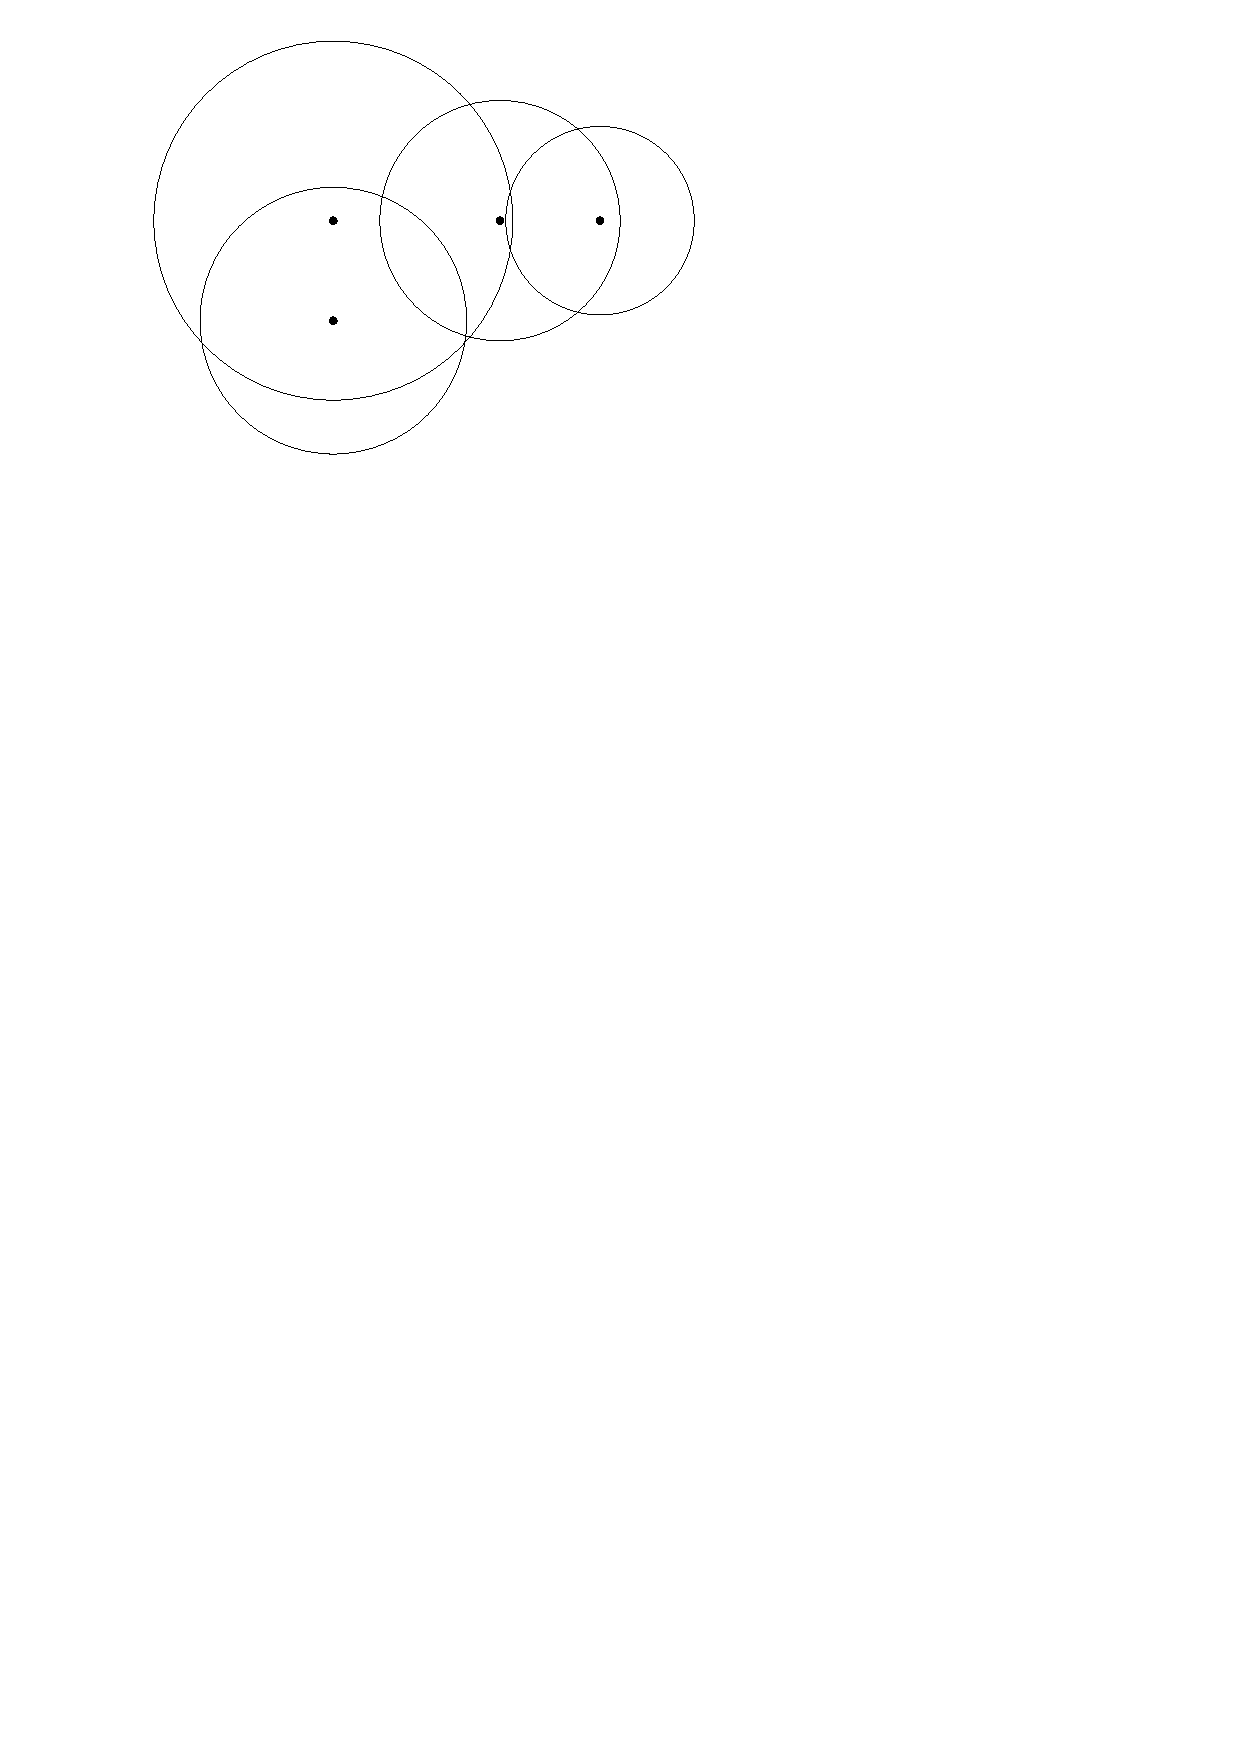
\includegraphics[scale=0.7]{figures/transmissionrange.pdf}
\caption{Four nodes with different transmission ranges\label{figure:tr}}
\end{figure}
\begin{figure}[ht]
\center
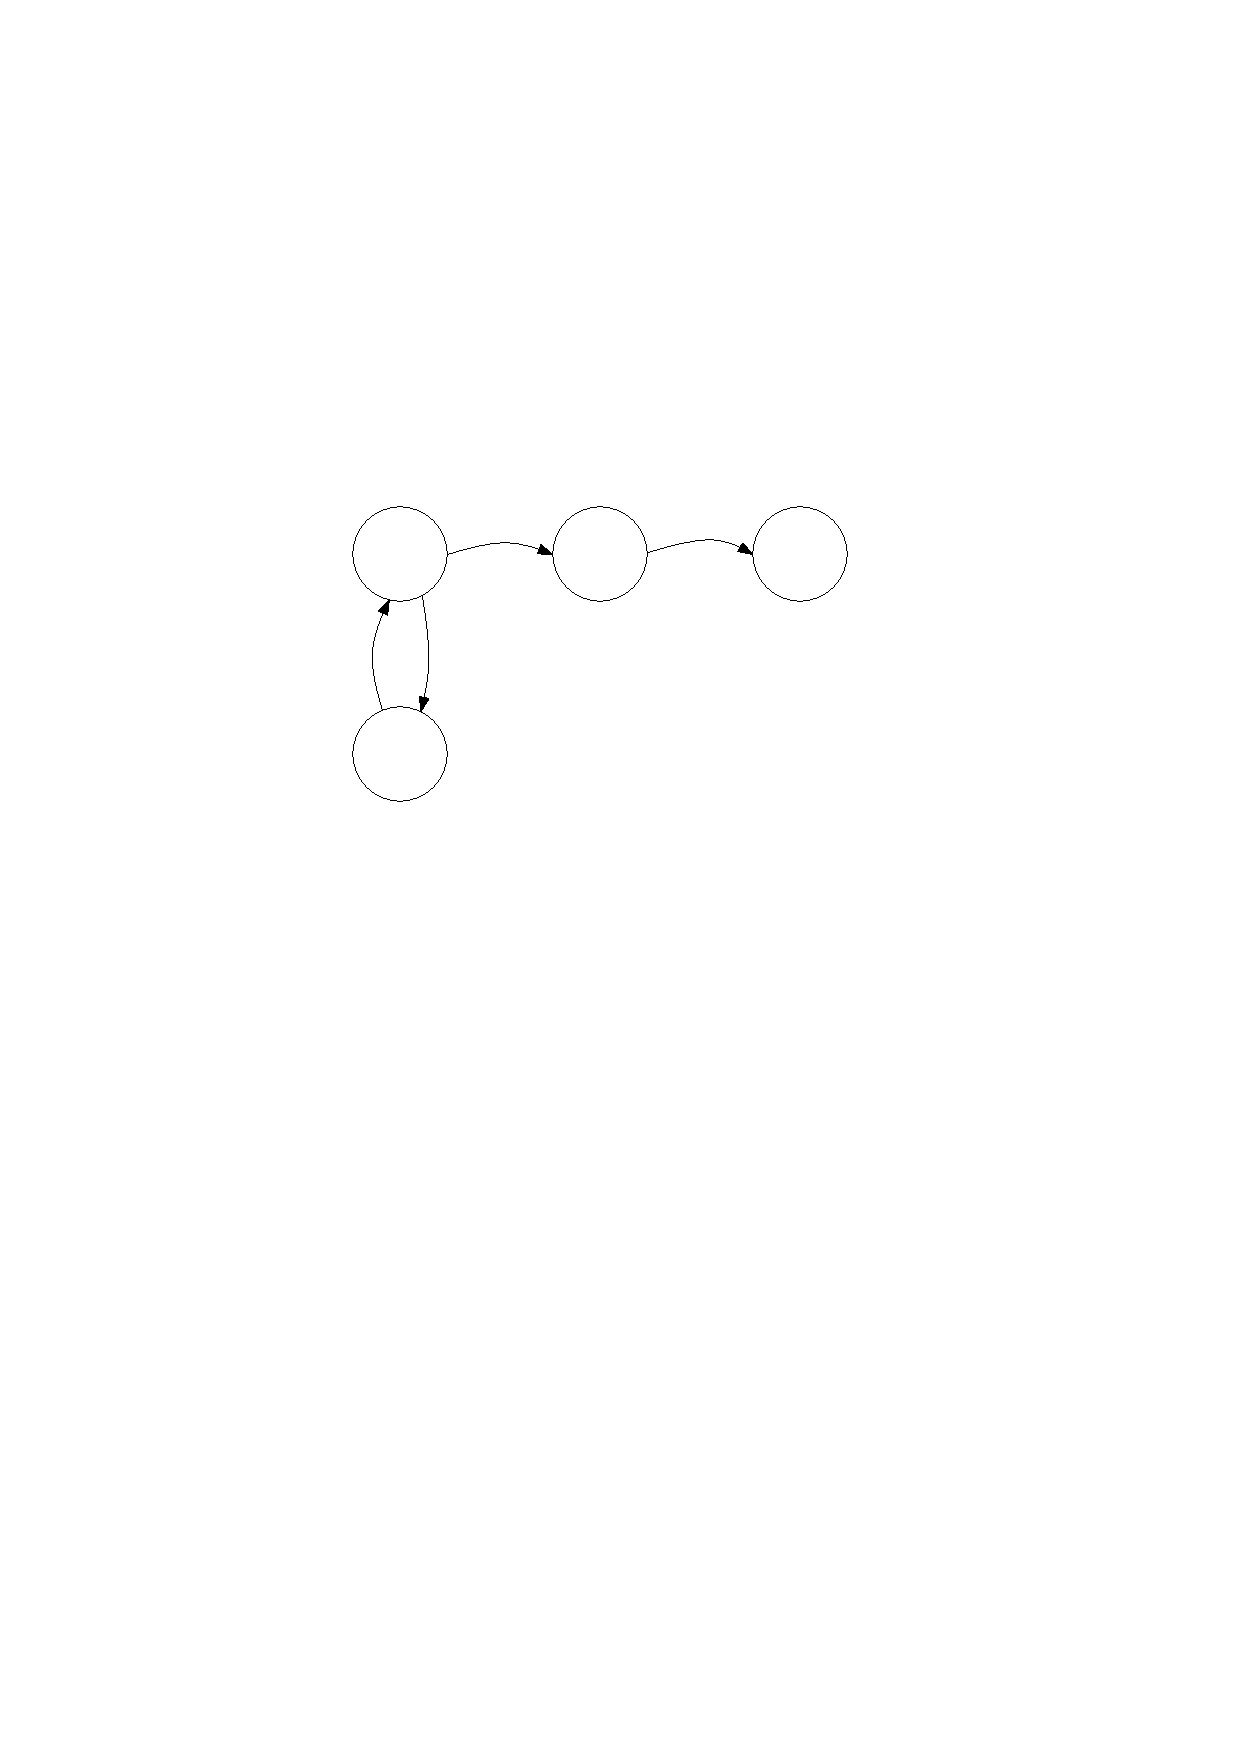
\includegraphics[scale=0.7]{figures/resultinggraph.pdf}
\caption{The communication graph resulting from Figure~\ref{figure:tr}}
\end{figure}


A \textit{Cycle} is defined as a finite set of edges $C \subseteq E$ so that you can construct a simple path $(u, v, \dots, u)$ from any starting edge $\in C$. Any bidirectional communication in our graph model is a cycle of length 2. Additionally we will introduce \textit{Strictly Directed Cycles}. These are cycles defined as before with an additional restriction: for any edge $(v, u) \in C$ it must hold that $(u, v) \notin E$.

\begin{lemma}
	In a disk graph, there are no strictly directed cycles.
\end{lemma}
\begin{proof}
	A strictly directed path $(u, v, \dots, w)$ implies that the transmission range $T_r(v)$ of each following node is smaller than the range of the node before it:
	$T_r(u)>T_r(v)>\dots>T_r(w)$. A cycle implies that the last node equals the first node ($u=w$), which would result in $T_r(u) > T_r(u)$ which is obviously impossible.
\end{proof}


\begin{figure}[ht]
\center
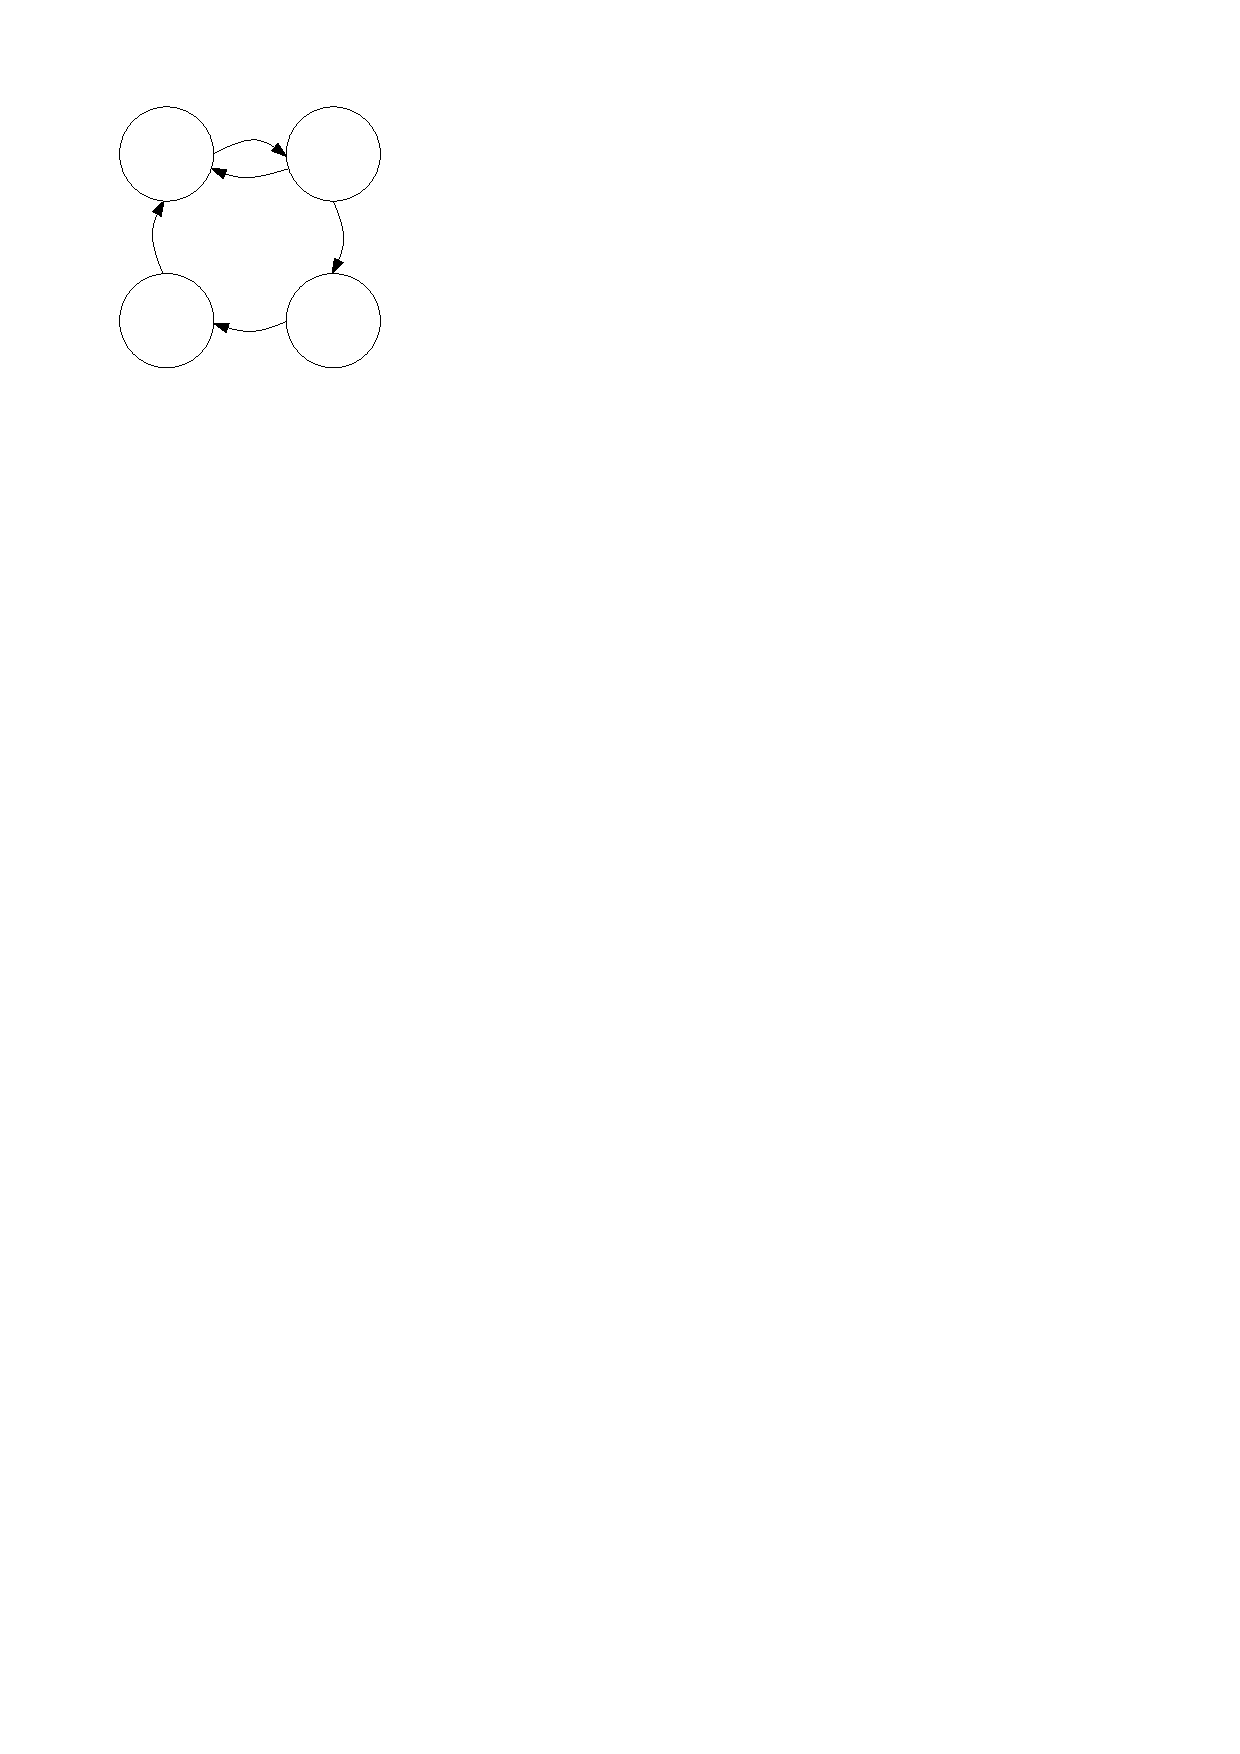
\includegraphics[width=0.2\linewidth]{figures/normalcycle.pdf}%
\hspace{2cm}
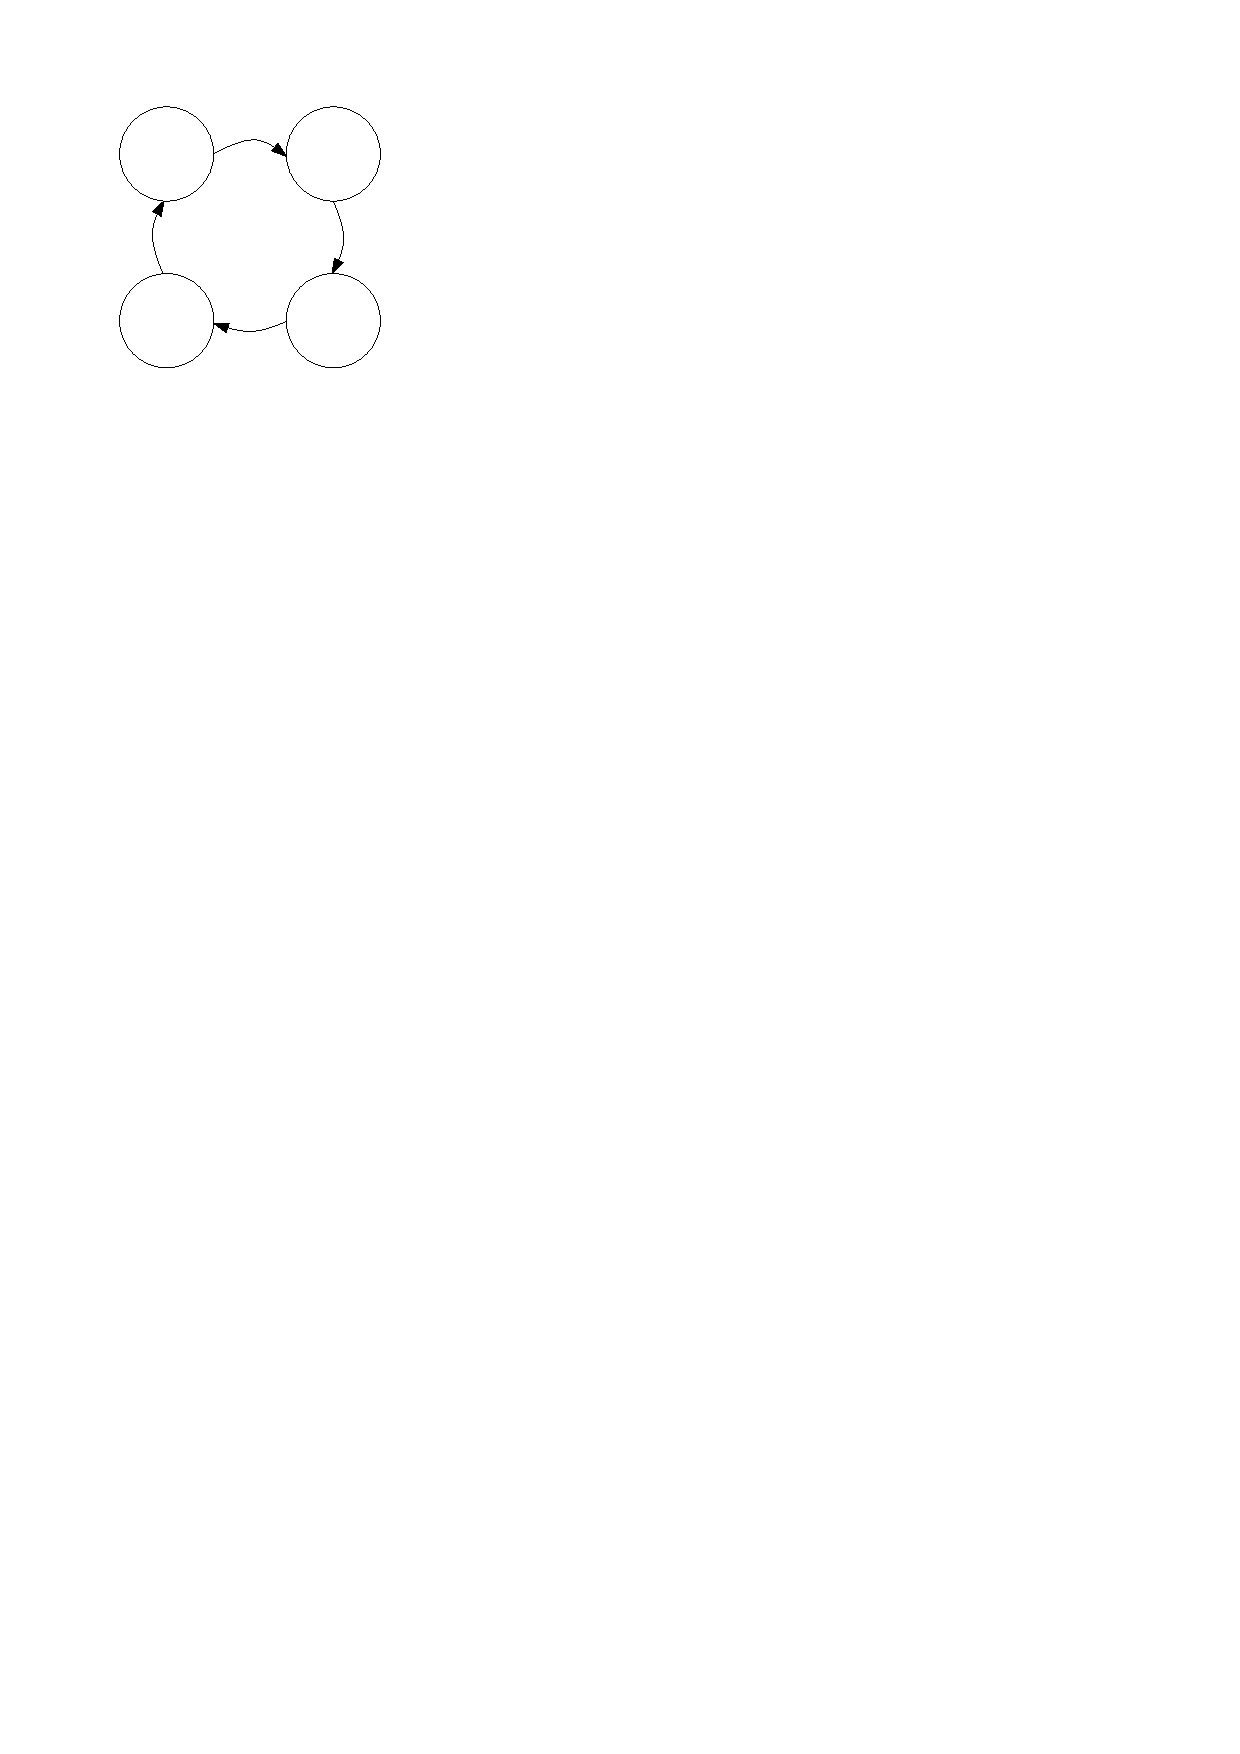
\includegraphics[width=0.2\linewidth]{figures/strictlydirectedcycle.pdf}%
\caption{Left: Graph containing two cycles, yet no strictly directed cycle. \\Right: Graph containing one strictly directed cycle.}%
\end{figure}

As these directed cycles are not possible in this model, we will work with the assumption that they do not exist in this thesis. However, in reality, this scenario could occur. At the end of the thesis, we will discuss the implications of these cycles on our algorithms.

One parameter which will be used often throughout this thesis is the parameter $l$, which describes the length of the longest strictly directed path $P$: $l = |P|+1$. This parameter, which is essentially 1 in unit disk graphs, influences the runtime of algorithms in this model, as we show in the proof of Algorithm~\ref{alg:r2d}.
%% content.tex
%%
\chapter{Randomized Algorithms With Initialization}
\label{ch:randomizedAlgorithms}

The following algorithms work using the CONGEST model. This means that we design the algorithm to operate as described in Section~\ref{section:comm}. The time for a local broadcast round can depend on several factors, most importantly on which communication model is used, then on whether the degree $\Delta$ is known. We generally assume for our nodes to have this knowledge.

The family of algorithms we work on in this thesis is randomized, which means that proof and run time analysis is generally coupled with high probability, which is defined as a probability of at least $1-1/n^c$ for an arbitrarily large constant $c$.

Nodes randomly select a color from the set of their available colors at a certain round, and then send it to their neighbors. If no collisions are detected, a node will keep that color and terminate, at which point the neighbors permanently respect that that color is taken and will not terminate using it. We will then reduce the number of colors by incorporating a coin tossing mechanism as described by Luby's distributed MIS algorithms in \cite{luby1986simple} and \cite{luby1988removing}.

The distributed graph coloring algorithms suggested Derbel and Talbi \cite{dt-dncsi-10}, while formally built on the SINR model, restric the graph to uniform disk graphs. As we showed in Section~\ref{section:graph}, modern models suggest a communication graph with directed edges instead, which has so far only been taken into consideration by Fuchs and Wagner \cite{DBLP:journals/corr/FuchsW14}. We shall present an algorithm which is simpler and uses less colors and iteratively improve on it throughout the thesis.

In this chapter, we shall take the Algorithm 18, from the monograph of Barenboim and Elkin \cite[p. 101]{be-dcg-13}, and add an initialization to discover dominators of nodes and add a new termination-condition for nodes so that nodes cannot terminate before their dominators do. This ensures that a node which has an outgoing one way communication link doesn't choose a color which would conflict with the color of an aleady terminated node. For the initialization phase, we introduce a helper algorithm which reveals to a node its $K$-neighborhood.


\begin{algorithm}[ht]
\DontPrintSemicolon 
\caption{\textsc{Get-K-Neighborhood(G)}}\label{alg:k-nghbr}
\SetKwFor{ForAll}{for}{do}

$N^0_v \defines (v, \emptyset)$\;

\ForAll{$i = 1 \dots K$}
{

\SetKwFor{ForEach}{for each}{do}

	send $N^{i-1}_v$\;

	$T = \emptyset$ \;

\ForEach{$N^{i-1}_u$ received}
{

$T = T \cup \{N^{i-1}_u\}$\;

$N^{i}_v \defines (v, T)$\;


}


}

return $N^k_v$

\end{algorithm}


This algorithm makes the $K$-neighborhood of a node known to that node. Its runtime depends on how many hops worth of neighborhood one needs to discover, which is represented by the parameter $K$. Each round, starting from round $i = 0$, a node sends out its own id plus the neighborhood it has discovered so far. This whole package is contained in the tuple $N^{i}_v$, with its first item being the node id, the second item being the set of packages $N^{i-1}_u$ for all neighbors $u$ of $v$.

\begin{lemma}
The Algorithm~\ref{alg:k-nghbr} takes $O(\Delta^{K-1})$ rounds to complete.
\end{lemma}
\begin{proof}
We prove this by doing a proof by induction over the parameter $K$.

For $K=1$, a node simply sends its own id too all of its neighbors, which is one round worth of communication.

For any $K > 1$, we see that the algorithm constructs $N^{K}_v$ out of $(v, T)$, with $T = \{N^{K-1}_u\}$ for all neighbors $u$ of $v$. So $T$ contains at most $\Delta$ times $N^{K-1}_u$. Sending all this data corresponds to at most $\Delta$ times the algorithm $\textsc{Get-(K-1)-Neighborhood(G)}$ being run, resulting in a run-time of at most $\Delta \cdot O(\Delta^{K-2})$ by the induction hypothesis. 
\end{proof}

\section{The Basic Algorithm (Rand-2-Delta)}

\begin{algorithm}[ht]
\DontPrintSemicolon 
\caption{\textsc{Rand-2-Delta}}\label{alg:r2d}

Run Get-$2$-Neighborhood \;
Let $D_v$ be the set of nodes that dominate $v$, calculated from $v$'s 2-neighborhood\;

Let $T_v = \emptyset$, the set of temporary colors of the neighbors of $v$\;
Let $F_v = \emptyset$, the set of final colors of the neighbors of $v$\;
Let $N_v = \emptyset$, the set of neighbors of $v$ which have terminated\;

\SetKwFor{ForEach}{for each}{do}

\ForEach{round}{
	$T_v = \emptyset$\;
	$c_v :=$ draw a color from $[2\Delta]$ randomly\;
	send the color $c_v$ to all neighbors\;
	\ForEach{received color $c_u$ from a neighbor $u$}{
		$T_v = T_v \cup \{c_u\}$\;
	}
	\If{$c_v \notin T_v \cup F_v$ and $D_v \subseteq N_v$\label{line:condition}}{
		send the message "final $c_v$" to all neighbors\;
		select $c_v$ as the final color of $v$ and terminate\;
	}
	\Else{
		\ForEach{received message "final $c_u$" from a neighbor $u$}{
			$F_v = F_v \cup \{c_u\}$\;
			$N_v = N_v \cup \{u\}$\;
		}
		discard $c_v$ and continue to the next round
	}
}

\end{algorithm}

At first we detect the local neighborhood of a node $v$ by broadcasting its identity, and then broadcasting all identities that $v$ has received. That way we know which nodes we can receive but not send to, which we save to $D_v$. Until all nodes in $D_v$ have terminated, $v$ only superficially joins the rounds of picking colors, as it never terminates before then. In each round, $v$ picks a random color from the pool $[2\Delta]$ and broadcasts it. If no neighbor picked the same color in the round or terminated with that color previously, and if $D_v$ is terminated, $v$ sends out the chosen color as "final $c_v$" and stops. By waiting for $D_v$ to be terminated, we ensure that every neighbor which cannot recieve that "final $c_v$" has already finished, and thus guarantee that no neighbor picks the same color, producing an invalid coloring.

We prove that the algorithm produces a valid coloring by proving that, when all nodes terminated, the graph has a valid coloring, and then proving that, with the runtime $O(\Delta \cdot l \log n)$, all nodes terminate with high probability by constructing a subgraph family and showing that it iteratively terminates until the whole graph terminated.

\begin{lemma}
\label{theorem:r2dproof}
  Algorithm Rand-2Delta produces a legal $2\Delta$-vertex-coloring when all nodes terminate.
\end{lemma}
\begin{proof}
  Let us choose a pair of neighbors arbitrarily, $u,v \in V$. Let $i,j$ be the rounds in which these nodes terminate respectively.
	
	\textbf{case } $i < j$: \\
	We also look at $j < i$ in this case by simply switching the roles of $u$ and $v$.\\
	For contradiction we assume that final $c_v = $ final $c_u$ and look at additional subcases:
	
	\begin{myindent}{3em}
	\textbf{case } $u$ dominates $v$: \\
	In the case that $v$ is dominated, it only chooses a final color when $u$ has chosen its final color, and $v$ cannot end with the same color (Line \ref{line:condition}).
	
	\textbf{case } $v$ dominates $u$: \\
	Directly contradicts $i < j$, as $v$ will terminate before $u$ (Line \ref{line:condition}).
	
	
	\textbf{case } $v$ and $u$ communicate: \\
	As $u$ terminates before $v$ does, $v$ knows "final $c_u$" is taken and cannot terminate using that (Line \ref{line:condition}) .
	\end{myindent}
	
	\textbf{case } $i = j$: \\
	In this case, both nodes terminate at the same time. As Line \ref{line:condition} requires that no neighbor of a node has the same color for the node to terminate (either temporary or finalized), $c_u \neq c_v$ and both nodes terminate with different colors.
\end{proof}

\begin{lemma}
\label{theorem:r2dzeit}
	Let $G_1$ be the subgraph of G, that contains all nodes that are not dominated by another node. Formally, $G_1 \defines (V_1 \defines \{v \in V : D_v = \emptyset \}, E(V_1))$. Algorithm \ref{alg:r2d} will produce a valid coloring for $G_1$ in $O(\log n)$ rounds, with a probability over $1-1/n^{c+1}$ for an arbitrarily large constant $c>1$.
\end{lemma}
\begin{proof}
	Similarly to Barenboim and Elkin \cite[p. 102]{be-dcg-13}, we argue that for a given node $v \in V_0$, the probability that it has chosen a color of one of its neighbors is at most $\Delta / 2\Delta$, the maximum number of neighbors divided by the size of the pool to choose its color from.
	
	Consequently, the probability that $v$ has not finished in round $i$ is $(1/2)^i$. By the union bound, the probability that such a $v$ exists for a given round $i$ is at most $n \cdot (1/2)^i$. \footnote{We could argue that instead of $n$, the number of nodes in the subgraph, $m = |V_1|$ suffices here.  However, as $m \leq n$, we will be using $n$ hereafter to simplify the proof.}  Hence, after $(c+2) \cdot \log n$ rounds, with probability not less than $1-n \cdot (1/2)^i \geq 1-1/n^{c+1}$, all of these nodes terminate successfully.
\end{proof}

We shall define a family of subgraphs which can be thought of a layer system. The first subgraph consist of the nodes which can be terminate freely, or in other words, are not dominated. We define $G_{k+1}$ as the subgraph, that includes all nodes which are dominated only by nodes of $G_k$, so for each iteration of $G_k$, one more layer of nodes are added. These layers will terminate one after another by the nature of this algorithm, so we prove the run time of the whole algorithm by proving the run time of each iteration.

\begin{definition} $G_0 \defines (\emptyset, \emptyset)$, 
$G_{k+1} \defines (V_{k+1} \defines \{v \in V : D_v \subseteq V_k\}, E(V_{k+1}))$.
\end{definition}
This family holds an invariant: $V_k \subseteq V_{k+1}$. An example of this family is shown in Figure~\ref{graphs}

\begin{figure}
\centering
\subcaptionbox{$G_1$\label{graph:g1}}[.49\linewidth]
{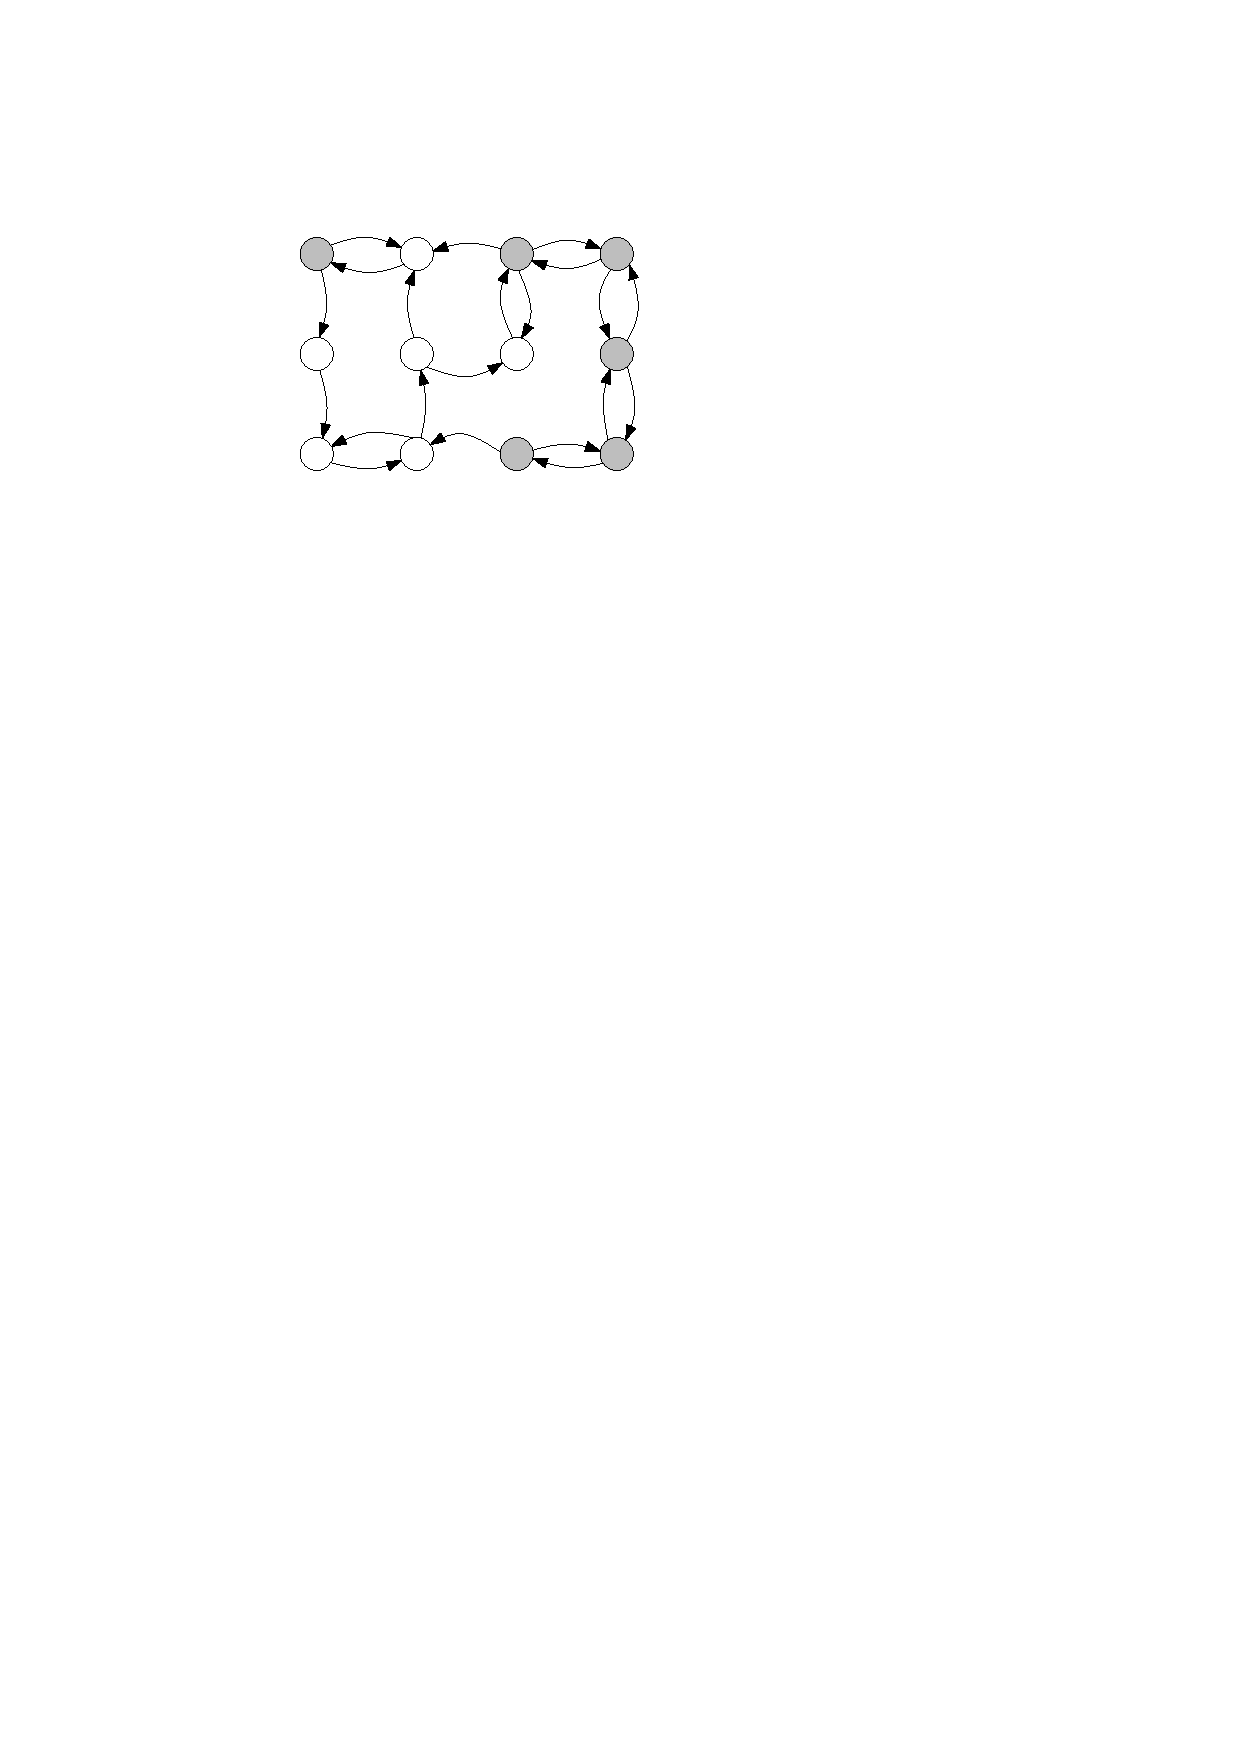
\includegraphics{figures/G_1.pdf}}
\subcaptionbox{$G_2$\label{graph:g2}}[.49\linewidth]
{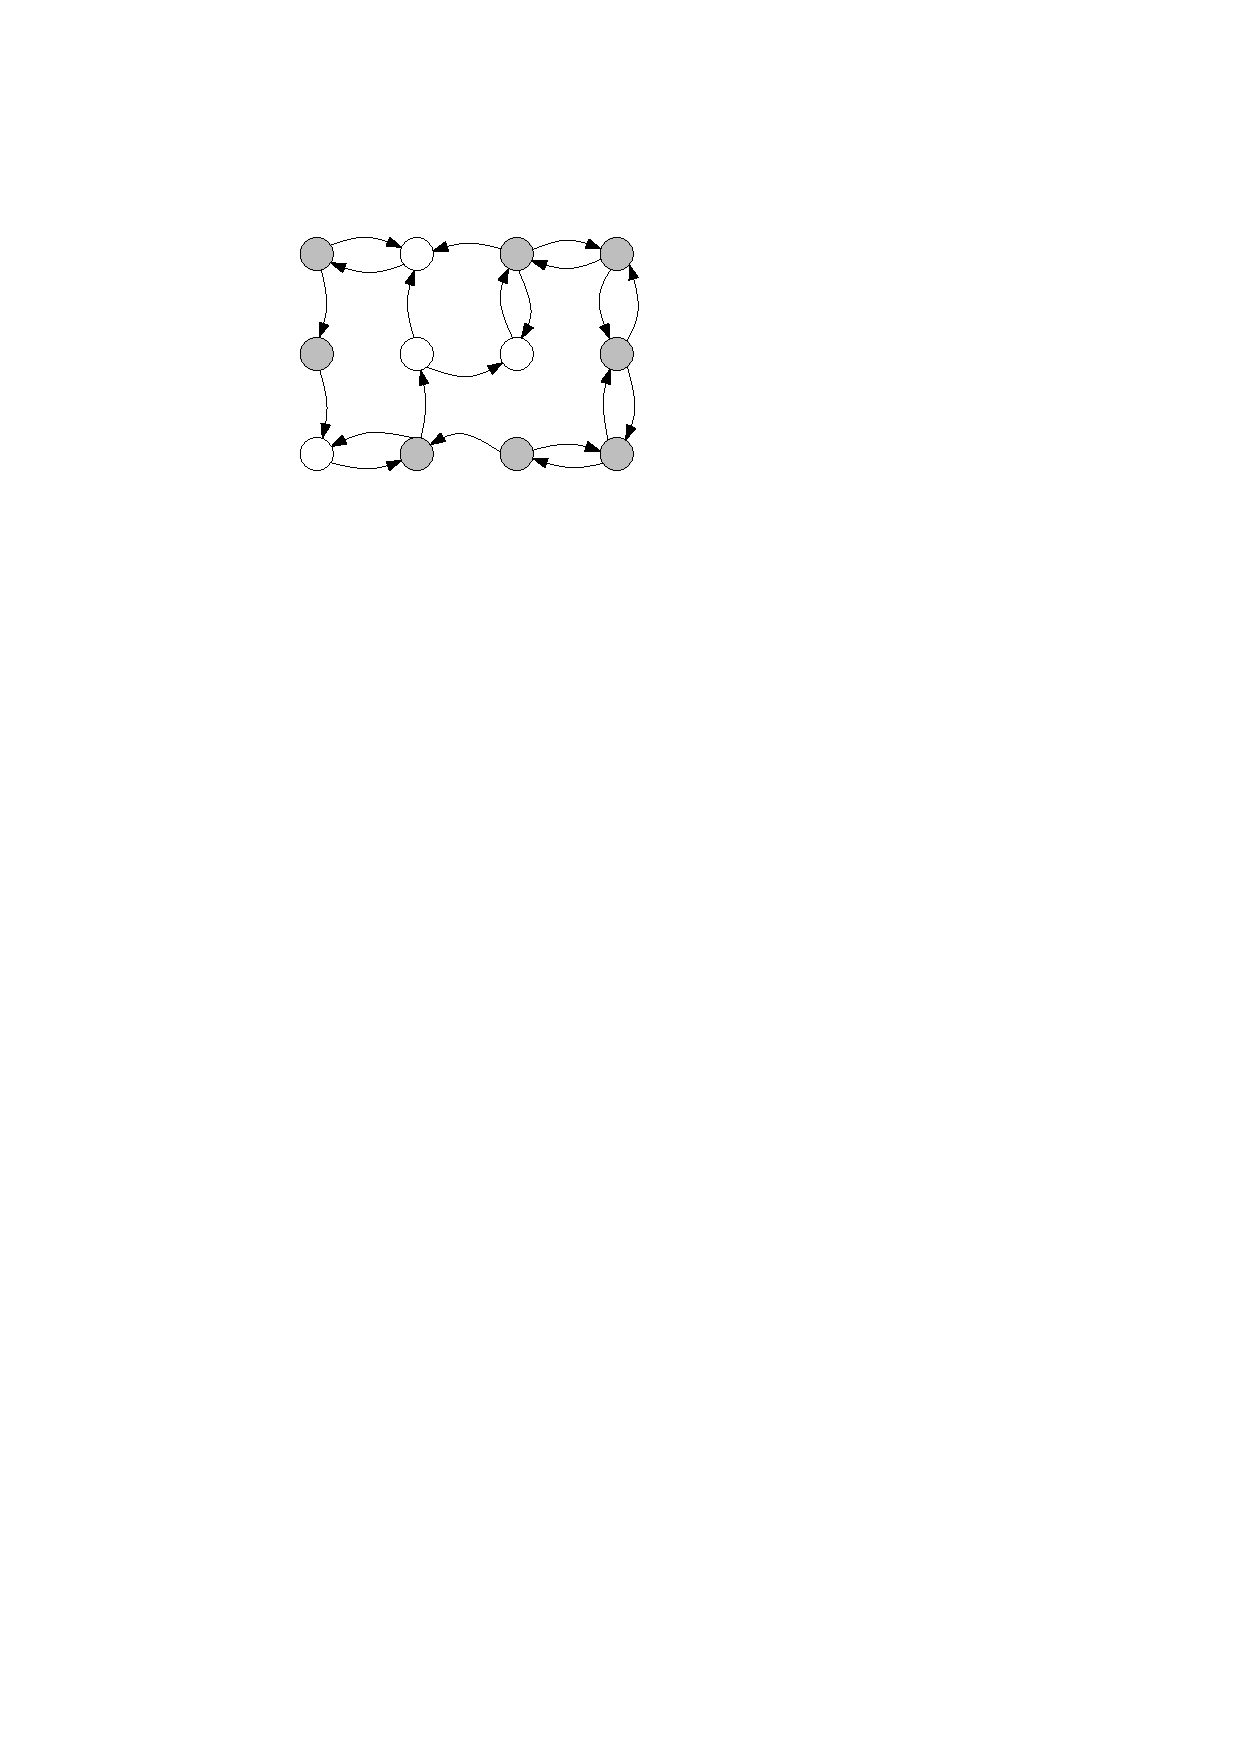
\includegraphics{figures/G_2.pdf}}
\subcaptionbox{$G_3$\label{graph:g3}}[.49\linewidth]
{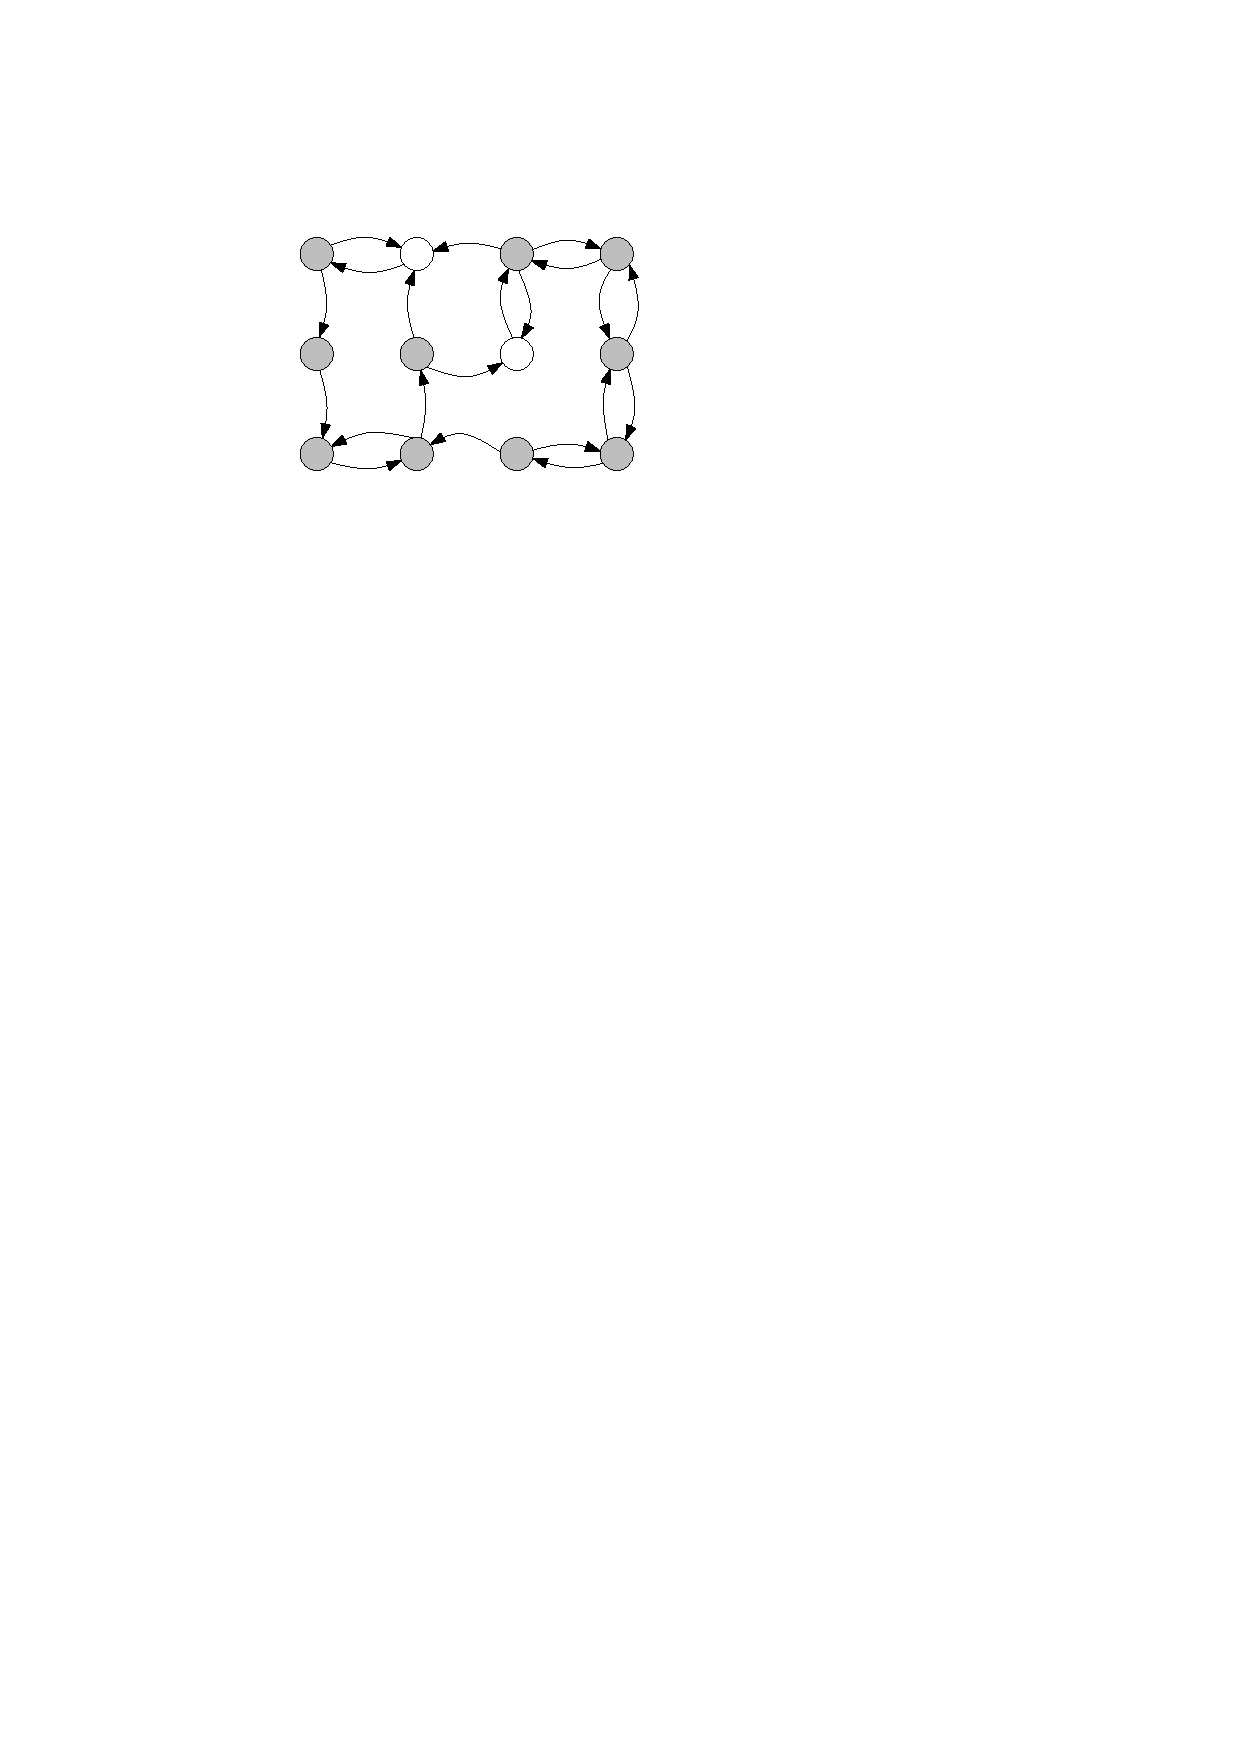
\includegraphics{figures/G_3.pdf}}
\subcaptionbox{$G_4 = G$\label{graph:g4}}[.49\linewidth]
{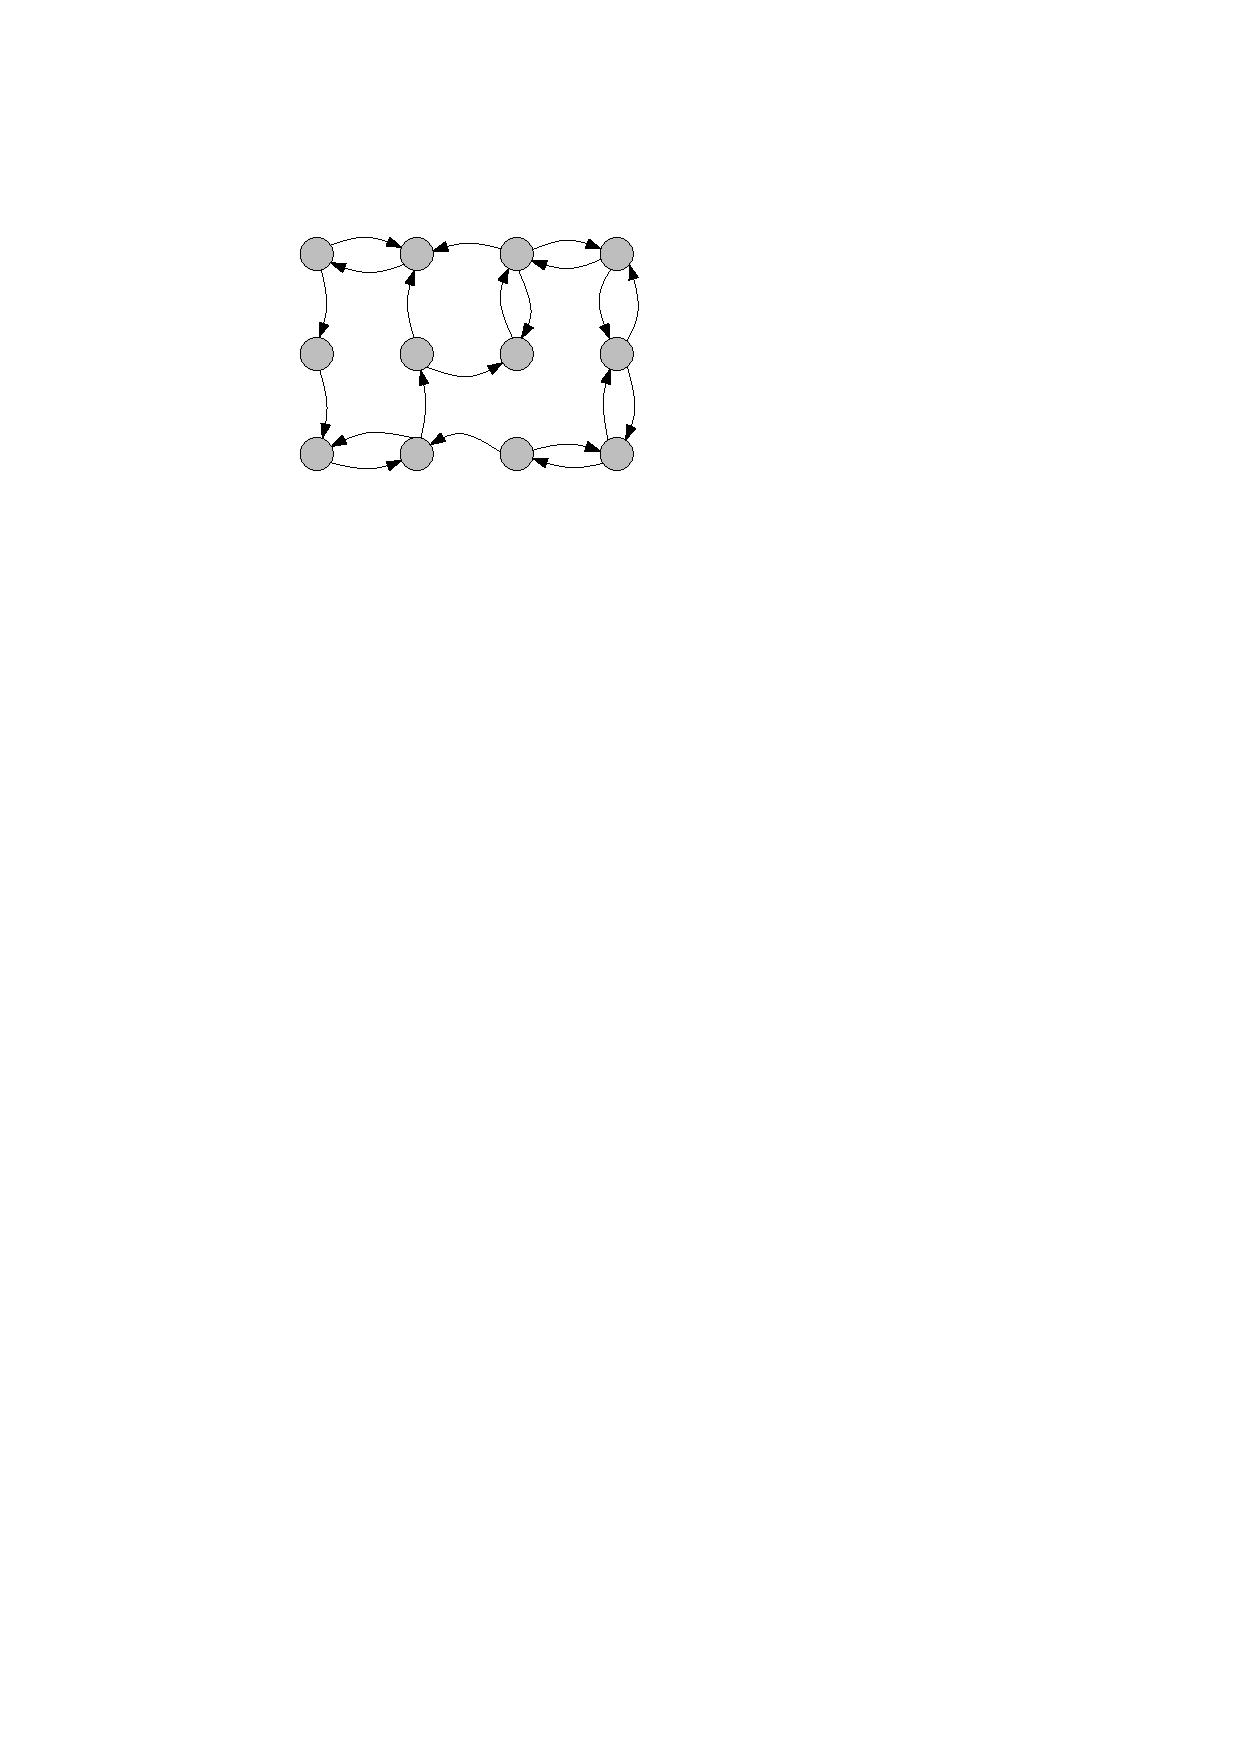
\includegraphics{figures/G_4.pdf}}
\caption{An example graph and its subgraph family $G_k$. In each iteration, all nodes which are only dominated by nodes from the previous iteration are added to the set.}
\label{graphs}

\end{figure}


\begin{lemma}
\label{theorem:r2dlaenge}
	$\exists N \in  \mathbb{N} : \forall k \geq N : G_k = G$.
\end{lemma}
\begin{proof}
	Let us choose $k$ so that $G_k = G_{k+1}$, it is sufficient to show that in that case $G_k = G$ already.
	Assume for contradiction that $G_k \neq G$. This means that in round $k+1$, no new nodes get added to the subgraph, so $V_k = V_{k+1} \neq V$. 
	
	We define $C \defines V \backslash V_k$ as the set of nodes which are not being added to the subgraph family, $C \neq \emptyset$. For an arbitrary node $v \in C$ this means that $D_v \cap C \neq \emptyset$, as $D_v$ contains at least one node $u$ that isn't in $V_k$.
	
	This implies that $|C| \geq 3$, since two nodes cannot dominate each other (that would be simply bidirectional communication). As for a given node $v$, we always have a node $u \in C$ which dominates it and therefore we can hop indefinitely to the next dominator. As we can do more than $|C|$ hops, this implies that $C$ contains a strictly directed cycle.
	
	This contradicts the definition of our graphs in Section~\ref{section:graph}.
\end{proof}

We shall now formally define the parameter $l$, which has been informally mentioned throughout the thesis so far.

\begin{definition}\label{definition:length}
Let $l$ be the smallest $k$, for which $G_k = G$ and $l-1$ be the length of the longest, strictly directed path in $G$.
\end{definition}

We discuss what happens when a strictly directed cycle is added to our communication graph in Section~\ref{lemma:cycles}, but obviously we cannot have an $l$, then, as the length of the longest, strictly directed path in that case is infinite, and $G_k \neq G$ for all $k \in \mathbb{N}$.

\begin{lemma}
\label{theorem:r2diteration}
	For a legally colored $G_k$, Algorithm \ref{alg:r2d} needs, with probability over $1-1/n^{c+1}$ for an arbitrarily large constant $c>1$, $O(\log n)$ rounds to legally color $G_{k+1}$.
\end{lemma}
\begin{proof}
	If $G_k = G$ we're already done.
	So we assume $G_k \neq G$.\\
	We choose a node $v$ out of the set $V_{k+1}\backslash V_k$ arbitrarily. Similarly to the first iteration, we argue that the probability for $v$ to still conflict with other nodes, and so to not being finished in round $i$ is at most $(\Delta /(2\Delta))^i = (1/2)^i$. We turn that around and argue that the probability for such a $v$ to exist in round $i$ is at most $n (1/2)^i$, and again after $(c+2) \cdot \log n$ rounds, with probability not less than $1-n \cdot (1/2)^i \geq 1-1/n^{c+1}$, all of these nodes terminate successfully.
\end{proof}

We conclude that

\begin{theorem}
\label{theorem:r2dkomplett}
	Algorithm \ref{alg:r2d} needs, with probability not less than $1-1/n^c$ for an arbitrarily large constant $c>1$, $O(\Delta + l \cdot \log n)$ rounds to terminate successfully.
\end{theorem}
\begin{proof}
	The sub-procedure Get-$2$-Neighborhood requires $O(\Delta)$ rounds to complete, as shown earlier. Combining the three previous lemmas, we need $O(\log n)$ rounds to compute $G_1$, then we need $l$ times $O(\log n)$ rounds to for all nodes in $G_l = G$ to terminate, at which point all nodes are legally colored. Each subgraph iteration from $G_{k-1}$ to $G_k$ has a probability over $1-1/n^{c+1}$ to finish with a valid coloring, we now simply union bound over all nodes to have all nodes terminate with a probability over $1-1/n^c$.
\end{proof}

\section{Color Reduction (Rand-Delta-Plus1)}

We can reduce the required amount of colors to $\Delta+1$ by letting nodes sleep with a probability of $1/2$, otherwise the algorithm still functions the same way: Every round, if a node doesn't sleep that round, it selects a color at random, sends it to all neighbors, and if there are no conflicts and all dominators have previously terminated, the node finalizes that color. By not having all nodes competing every round, we lower the chance for the nodes to pick conflicting colors, which enables us to reduce the amount of colors while keeping the same asymptotical run-time. $\Delta+1$ colors is what is aimed for in graph coloring algorithms and is the best possible amount of colors for algorithms coloring arbitrary graphs.


\begin{algorithm}[ht]
\DontPrintSemicolon 
\caption{\textsc{Rand-Delta-Plus1}}\label{alg:rd+1}

Run Get-$2$-Neighborhood \;
Let $D_v$ be the set of nodes that dominate $v$, calculated from $v$'s 2-neighborhood\;

Let $T_v = \emptyset$, the set of temporary colors of the neighbors of $v$\;
Let $F_v = \emptyset$, the set of final colors of the neighbors of $v$\;
Let $N_v = \emptyset$, the set of neighbors of $v$ which have terminated\;

\SetKwFor{ForEach}{for each}{do}

\ForEach{round}{
	$T_v = \emptyset$\;
	$c_v =$ draw from $\{0,1\}$ randomly\;
	\If{$c_v = 1$}
	{
	$c_v =$ draw a color from $[\Delta+1]$ randomly\;
	send the color $c_v$ to all neighbors\;
	\ForEach{received color $c_u$ from a neighbor $u$}{
		$T_v = T_v \cup \{c_u\}$\;
	}\;
	\If{$c_v \notin T_v \cup F_v$ and $D_v \subseteq N_v$}{
		send the message "final $c_v$" to all neighbors\;
		select $c_v$ as the final color of $v$ and terminate\;
	}
	}
	
		\ForEach{received message "final $c_u$" from a neighbor $u$}{
			$F_v = F_v \cup \{c_u\}$\;
			$N_v = N_v \cup \{u\}$\;
		}
		discard $c_v$ and continue to the next round
}

\end{algorithm}

This algorithm also initializes before beginning the main loop to get the neighborhood information for a node and from that which neighbors dominate it. It then tosses a coin and if it wins, it randomly draws colors and compares them to the neighbors which also drew colors, and if no collisions happen \textit{and} if all dominating neighbors have terminated, the node terminates with its most recent color.

\begin{lemma}\label{lemma:rd+1iteration}
	Given that $G_k$ has terminated, Algorithm~\ref{alg:rd+1} needs $O(\log n)$ rounds for $G_{k+1}$ to terminate with high probability.
\end{lemma}
\begin{proof}
	Given a node $v$ for which all neighbors in $D_v$ have terminated and given that it currently has a conflicting color and does not terminate in the current round, the probability that it has a conflict with one given neighbor in the next round is at most $\frac{1}{2\cdot(\Delta+1-|F_v|)}$ after the coin toss. $1/2$ is the probability for the neighboring node to activate.
	
	When we union bound this probability over all neighbors, the chance that $v$ conflicts in the next round, given that the coin toss succeeds, is at most $(\Delta+1-|F_v|) \cdot \frac{1}{2 \cdot (\Delta+1-|F_v|)} = \frac{1}{2}$. Thus the probability that $v$ finishes in the next round is $1/2 \cdot 1/2 = 1/4$ and the probability that it has not finished after $i$ rounds is $(1-1/4)^i = (3/4)^i$. We union bound it over all nodes to argue that the probability of a node that hasn't terminated yet is $n\cdot (3/4)^i$.
	
	After $i=(c+2)\cdot 4\log n$ rounds, with a probability of at least $1-n\cdot (3/4)^i \geq 1-1/n^{c+1}$ no more nodes are in conflict and thus all terminated.
\end{proof}

We will now simply use $G_0$ for the induction start instead, which is trivial as all nodes in $G_0$ are terminated and then re-use Lemmas~\ref{theorem:r2dproof},~\ref{theorem:r2dlaenge} and \ref{lemma:rd+1iteration} to show that:

\begin{theorem}
	Algorithm~\ref{alg:rd+1} produces a valid $\Delta+1$ coloring in $O(\Delta + l \log n)$ with high probability.
\end{theorem}
\begin{proof}
	For each subgraph $G_k$ with $k \in \{1\dots l\}$ the algorithm needs $O(\log n)$ rounds to color it, as seen in Lemma~\ref{lemma:rd+1iteration} with probability $1-1/n^{c+1}$. As in Theorem~\ref{theorem:r2dkomplett} we union bound that to say $G_l$ is terminated with probability $1-1/n^c$ after $O(l \log n)$ rounds. Add the initialization and with Lemma~\ref{theorem:r2dlaenge}, $G$ is colored after $O(\Delta + l \log n)$ with high probability.
\end{proof}


\chapter{Without Initialization}

In order to get rid of the $\Delta$-summand (which can get quite large, see Figure~\ref{fig:boxplotndelta}) in the run-time of Algorithm~\ref{alg:r2d}, we will need, of course, to remove the neighborhood-search, and to accomodate for the uncertainty a node now has, as it can never know whether it has terminated or if it could be forced to change its color in the future by a dominator. Because of this uncertainty, we have to increase the amount of possible colors from Algorithm~\ref{alg:r2d} by $\Delta$ to $3\Delta$.

\section{The Algorithm (Rand-3-Delta)}

\begin{algorithm}[ht]
\DontPrintSemicolon 
\caption{\textsc{Rand-3-Delta}}\label{alg:ir2d}

Let $T_v = \emptyset$, the set of colors of the neighbors of $v$\;

$c_v \defines$ draw a color from $[3\Delta]$ randomly\;

\SetKwFor{ForEach}{for each}{do}

\ForEach{round}{
	$T_v = \emptyset$\;
	send the color $c_v$ to all neighbors\;
	\ForEach{received color $c_u$ from a neighbor $u$}{
		$T_v = T_v \cup \{c_u\}$\;
	}\;
	

	\If{$c_v \in T_v$}
	{
		redraw $c_v$ from $[3\Delta] \backslash T_v$
		}\label{alg:ir2d:while}
}

\end{algorithm}

Algorithm~\ref{alg:ir2d} initially draws a color from $3\Delta$ and for each round, send its chosen color to all neighbors and it will only change its chosen color if it detected a collision in the current round.

It looks a lot simpler than Algorithm \ref{alg:r2d}, however the latter is easier to prove to be working correctly, and we will be using it as a stepping stone to prove the former.

Even though the nodes don't know the set of their dominating nodes $D_v$, for the proof we will still use this set as defined in Algorithm \ref{alg:r2d}. We will also use the family of subgraphs defined in \ref{theorem:r2dzeit}.

As nodes cannot enter the state \textit{terminated} anymore, because of their lack of knowing their dominating nodes, we will introduce the notion of a stable node. A node is \textit{stable} when it never changes its color in the future anymore. Obviously a node cannot know when it will be stable itself, but we can determine when it will be stable in the proof. We shall first prove that the graph has a valid coloring once all nodes are in the stable state, then we show when a node enters that state and prove that it indeed doesn't leave it, and then we use the subgraph family to iteratively prove the run-time, as in the previous algorithms.

\begin{lemma}\label{lemma:ir2d-proof}
	When all nodes are stable, Algorithm~\ref{alg:ir2d} has produced a legal $3\Delta$ coloring of $G$.
\end{lemma}
\begin{proof}
	Let us assume for contradiction that for two neighboring nodes $u$ and $v$, $c_u = c_v$, then either one (in case one is dominated by the other) or both nodes redraw their colors and hence are not stable.
\end{proof}

\begin{lemma}\label{lemma:ir2d-redraw}
	A node $v$ is stable when $D_v$ is stable and $v$ has stopped redrawing once since then.
\end{lemma}
\begin{proof}
	If we assume that $v$ did not need to redraw in round $i$, but needs to redraw in round $i+1$, which means that some other node $u$ picked the color $c_u = c_v$, it follows that either $v$ was dominated by $u$, in which case $u \in D_v$ should have been stable already, or $u$ picked $c_u \notin T_u$ which contradicts line~\ref{alg:ir2d:while}, since $c_v \in T_u$.
\end{proof}

\begin{lemma}\label{lemma:ir2d-zeit}
	The subgraph $G_1$, with high probability, is stable after $O(\log n)$ rounds.
\end{lemma}
\begin{proof}
	For an arbitrary node $v \in V_1$, the chance that it conflicts in the first round is $\Delta / 3\Delta = 1/3 < 1/2$. For each successive round, the pool of colors $v$ can choose from is at least $2\Delta$ as at most $\Delta$ colors may be blocked. In the worst case, all neighbors switch to a new color and the chance that $v$ is in a conflict again is at most $\Delta / 2\Delta = 1/2$, the number of all neighbors choosing a new color divided by their pool.
	
	As we did for Algorithm \ref{alg:r2d}, using Lemma \ref{lemma:ir2d-redraw} (as $D_v = \emptyset$, which obviously is stable), we can now argue that the chance for a node to not be stable in round $i$ is at most $1/2^i$ and by the union bound assert that the chance for such a node to exist is at most $n \cdot 1/2^i$. Again, after $(c+2) \cdot \log n$ rounds, with probability not less than $1-n \cdot (1/2)^i \geq 1-1/n^{c+1}$, there is no more such node.
\end{proof}

\begin{theorem}\label{theorem:ir2d}
	Algorithm \ref{alg:ir2d} produces, with high probability, a valid $3\Delta$-coloring of $G$ in $O(l \log n)$ rounds.
\end{theorem}
\begin{proof}
	As we showed before, we assert that for each iteration of $G_{k+1}$, it takes, with high probability, not longer than $O(\log n)$ rounds, as all dominating nodes of $G_{k+1}$ in $G_k$ are stable, the remaining nodes respect their chosen color and have, in the worst case, still at most $\Delta$ neighbors picking a new color. With that, again, we have the probability of a node $v$ having to redraw in round $i$ at most $(1/2)^i$, and use the same argument as before, finding that with high probability it takes $O(\log n)$ rounds to make $G_{k+1}$ stable. So, from Lemma~\ref{theorem:r2dlaenge} we can state that after $l \cdot O( \log n)$ rounds $G_l = G$ is stable and from Lemma~\ref{lemma:ir2d-proof} that Algorithm~\ref{alg:ir2d} indeed produced a valid coloring.
\end{proof}

\section{Color Reduction (Rand-2Delta-Plus1)}

Let us now improve this algorithm so that it works with $2\Delta+1$ colors. Unfortunately, without the knowledge of the dominating nodes, we cannot reduce the necessary colors to $\Delta+1$.

\begin{algorithm}[ht]
\DontPrintSemicolon 
\caption{\textsc{Rand-2Delta-Plus1}}\label{alg:r2d+1}

Let $T_v = \{0\}$, the set of colors of the neighbors of $v$\;
Let $c_v = 0$ be an invalid color\;

\SetKwFor{ForEach}{for each}{do}

\ForEach{round}{

	\If{$c_v \in T_v$}
	{
		draw $c_v$ from $\{0, 1\}$\;
		\If{$c_v = 1$}
		{
			redraw $c_v$ from $[2\Delta+1] \backslash T_v$
		}
		
	}
	
	$T_v = \{0\}$\;
	
	
	send the color $c_v$ to all neighbors\;
	\ForEach{received color $c_u$ from a neighbor $u$}{
		$T_v = T_v \cup \{c_u\}$\;
	}
	
	

}

\end{algorithm}

Algorithm~\ref{alg:r2d+1} introduces an invalid color $0$ and a node defaults to that color. In each round, if the node has the color $0$ or is in conflict with a neighbor, it will throw a coin and either choose the color $0$ or pick a random color from the colors $[2\Delta]\backslash T_v$, which are the currently unpicked colors. This will ensure that a node will not pick a color which is held by a stable node, which would force that stable node to redraw and so break its stability.


\begin{lemma}$G_k$ stabilizes with high probability after at most $O(\log n)$ rounds, given that $G_{k-1}$ is stable.
\end{lemma}
\begin{proof}
	For an arbitrary node $v \in V_k$, given that it draws a new color from its available pool ($[2\Delta+1] \backslash T_v$), the probability that it chooses a color that another neighbor $u$ chooses ($c_u = c_v$) is less than $\frac{1}{2\Delta+1- |T_v \backslash\{0\}|} \cdot \frac{1}{2}$, one out of the available colors times the chance that the neighbor picks something different from $0$, which is $\frac{1}{2}$.
	
	By the union bound over the neighbors of $v$, the chance that such a collision occurs is lower than
\begin{align*}
	(\Delta+1) \cdot \frac{1}{2 (2\Delta+1-|T_v \backslash\{0\}|)}\leq (\Delta+1) \cdot \frac{1}{2 (\Delta+1)} = \frac{1}{2}\hspace{1em}.
\end{align*}
	So if $v$ selects a new color, it is a distinct from all of its neighbors with a chance bigger than $1-\frac{1}{2}$. The chance that it becomes stable (see Lemma~\ref{lemma:ir2d-redraw}) is therefore at least $\frac{1}{2} \cdot \frac{1}{2} = \frac{1}{4}$ per round.
	
	Thus $v$ is not stable yet in round $i$ with a probability of at most $(1-\frac{1}{4})^i = \frac{3}{4}^i$ and by the union bound, such a node exists with a probability of at most $n \cdot \frac{3}{4}^i$.
	
	After $i = (c+1)\cdot 4\log n$ rounds, with probability greater than $1 - n \cdot \frac{3}{4}^i \geq 1-\frac{1}{n^c}$ no such node exists.
\end{proof}

\begin{theorem}
We conclude that a $2\Delta+1$ coloring will be calculated by Algorithm~\ref{alg:r2d+1} with high probability in $O(l \log n)$.
\end{theorem}


\chapter{Lower Bound and Outlook}

In this chapter, we introduce a lower bound to randomized graph coloring algorithms in directed graphs and discuss the consequences and a possible solution for strictly directed cycles.

\section{Lower Bound ($\Omega (\min\{l, \log n\})$)}

In this section we introduce a lower bound to randomized algorithms with bounded conflict probabilities solving directed graphs. We argue that the strictly directed path with length $l$ directly influences the run time of that algorithm asymptotically, at least up to $\log n$ rounds, at which point the algorithm could begin to have a high probability to have that path successfully colored.

\begin{theorem}\label{theorem:lowerbound}
For a randomized algorithm which produces valid $O(\Delta)$ colorings on any directed graph with high probability, there exists a lower bound of $\Omega (\min\{l, \log n\})$ rounds to compute it.

\end{theorem}
\begin{proof}
Let us look at a special kind of (sub)graph, a chain of single nodes dominating the next one. We will be using $v_1, \dots v_{l+1}$ to refer to the nodes.

\begin{figure}[ht]
\center
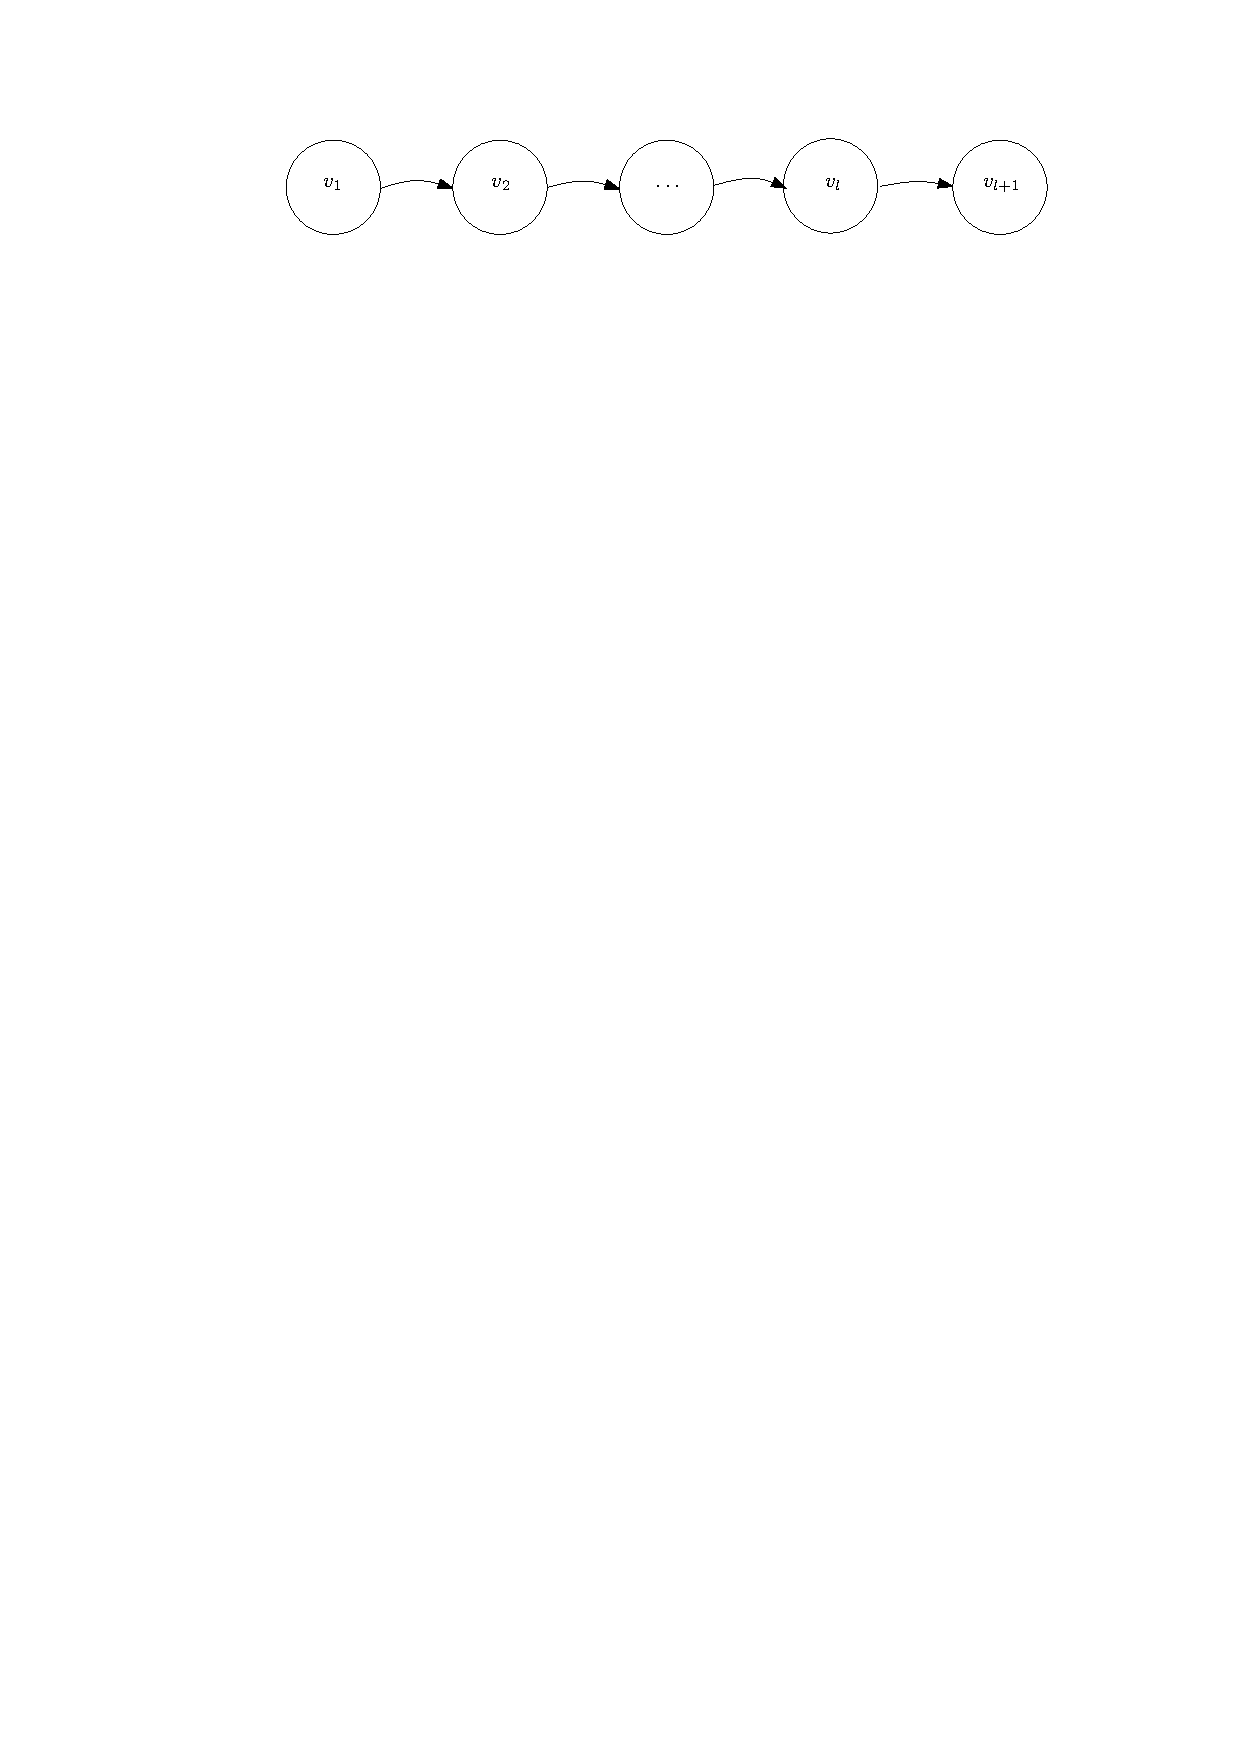
\includegraphics{figures/chain.pdf}
\caption{A graph consisting of a chain of dominating nodes}
\end{figure}

For each edge $(v_k, v_{k+1})$, each time $v_k$ picks a color, there is a probability that it produces a conflict as $v_{k+1}$ is dominated and $v_k$ therefore cannot respect the choice of that color. There exists a constant $c>1$ (for example $c \defines 2$ in Algorithm~\ref{alg:ir2d}) so that the probability for such a conflict is at least $1/c$ for every edge, and the probability that a conflict spreads $t$ hops is at least $1/c^t$.

Let us assume for contradiction that the runtime $T(n)$ of the algorithm is $\in o(\log n)$ with a probability of at least $1-1/n^{\tilde{c}}$ for a fixed constant $\tilde{c} > 1$.

It follows that $\exists N \in \mathbb{N} : \forall n > N$ it holds that $T(n) < \tilde{c} \cdot \log_c n$.

The probability that there is no conflict after $T(n)$ rounds is therefore 

\begin{align*}
1-\frac{1}{ c^{T(n)} } < 1- \frac{1}{c^{\tilde{c} \cdot \log_c n}} = 1- \frac{1}{n^{\tilde{c}}}.
\end{align*}

Which is a contradiction.

This means that the lower bound is $l$ for values asymptotically smaller than $\log n$, because on general graphs, $n$ can be extremely huge while the subgraph containing the longest, strictly directed path can be small, and $\log n$ for larger values of $l$, or $\Omega (\min\{l, \log n\})$.
\end{proof}


This bound should be seen as an addition to Linials bound \cite{linial1992locality}, which holds true for our algorithms, too. As such, we can combine the two bounds:

\begin{corollary}
	For a randomized algorithm which produces valid $O(\Delta)$ colorings on any directed graph with high probability, there exists a lower bound of $\Omega (\log^* n + \min\{l, \log n\})$ rounds to compute it.
\end{corollary}


\section{Strictly Directed Cycles}\label{lemma:cycles}

As an outlook, we indicate using the following argumentation, that the Algorithms \ref{alg:r2d}, \ref{alg:ir2d}, \ref{alg:rd+1} and \ref{alg:r2d+1} still create a valid coloring when a strictly directed cycle occurs, but the parameter $l$ will not formally exist the way we defined it in Definition~\ref{definition:length}.

We have argued before that if a strictly directed cycle exists, at some point a subgraph containing that cycle will not be added to the family of subgraphs $G_k$ anymore. Let $G_i$ be the biggest subgraph not containing the cycle and the nodes dominated by it, and let it be stable (or terminated). We will interpret the cycle as a path of infinite length.

After $(c+1) \cdot \log n$ rounds, with probability not less than $1 - 1/n^c$, no more conflicts are spreading through this cycle, using the same union bound as was used for conflicts in single nodes before, now we used it to bound the hops, as all nodes which are not stable yet either belong to that cycle, or are dominated by it, and as such the nodes do not generate collisions with neighbors outside of $C$ anymore.

We add the cycle $C$ to the subgraph $G_{i+1}$ and continue to construct the subgraph family until $G_l = G$.

This way, the algorithms would still find a correct coloring when a strictly directed cycle occurs. This discussion will then, once these cycles will actually be possible in a communication graph model, need to be formalized and proven for every constellation of cycles.


\chapter{Experimental Data}

In this chapter we look into experimental data about the size of the parameter $l$ in a more pratical setting. We shall also show correlations between other parameters. The motivation behind this is the question, whether this parameter has a neglectible impact on performance in practice, or if it is indeed an important factor in this graph model. We shall first describe the way we obtained the data, then we shall report the observations. In the last section, we discuss these observations and their impact.


\section{Setup}

We used a simulator written in the programming language $C\#$ using open source libraries such as QuickGraph\footnote{http://quickgraph.codeplex.com}. Our project is basically divided into two components: a webservice which is located in the cloud and acts as the central database to store the experimental data, and an executable which runs simulations sequentially and sends the results to the webservice. This executable could then be distributed on to several machines, to increase the numbers of parallel simulations. Note that these machines run independently, as the work gets distributed randomly instead of using sophisticated, deterministic work allocation schemes.


\subsection{Graph Construction}

The graph factory is a core component of the simulator. Its task is to generate random graphs within certain bounds. To make these graphs as closely aligned to the communication graph model we obtained from Section~\ref{section:graph}, we generate using the following geometric considerations.

Each node is given a random double-precision floating value between $0$ and $1$ for their $x$ and $y$-coordinates. Additionally, they are given a transmission range similarly to the SINR model, although we omit the intensive physical calculations that model involve and determine the ranges in a simpler way by defining an average range the nodes in the graph should have beforehand, together with a value of how much variance we want to allow, and then give each node a random range within these constaints.

The minimum range is defined as $0.005$ , whereas the average range that is chosen for each graph at random is a value between this minimum and $0.2$, then for each graph, a random value for maximum divergence is chosen between $1$ and $8$, we chose this relatively large value so that a single node could potentially, if it had the maximum range allowed, reach the whole graph. For each node generated, its range is calculated by creating a random double precision float between $MaxDivergence$ and $1/MaxDivergence$, which is then multiplied with the average range.

From this node set, we calculate the communication graph by using simple Euclidian distance calculations. For two nodes $u$ and $v$ and their distance $\dist(u, v)$, we add an edge $(u,v)$ if $\dist(u, v) < \range(u)$ and an edge $(v,u)$ if $\dist(u, v) < \range(v)$. The node count is bounded between $100$ and $10000$ and also chosen at random.

To produce graphical representations of the graphs we saved the data in the GraphML\footnote{http://graphml.graphdrawing.org} format, for which a multitude of renderers exist. We show some example graphs in the Appendix Section~\ref{appendix:graphs}.

\subsection{Analytics}


We collect, from each generated graph, a set of properties, which we shall statistically analyze in the next section. In Table~\ref{table} we describe the data that we collected.
\begin{table}[th]
\begin{tabularx}{\textwidth}{l|X}
NodeCount	& The number of nodes in this graph.\\
CriticalPathLength & The value of the parameter $l$.\\
AverageInDegree	& The average in-degree of all nodes.\\
AverageOutDegree		& The average out-degree of all nodes.\\
MaxInDegree	& The largest in-degree of all nodes.\\
MaxOutDegree	& The largest out-degree of all nodes.\\
WeaklyConnectedComponents	& The number of weakly connected graph components.\\
StronglyConnectedComponents	& The number of strongly connected graph components.\\
AverageRange	& the average transmission range of all nodes.\\
MaxRange	& The largest transmission range of all nodes.\\
MinRange & The smallest transmission range of all nodes.\\

\end{tabularx}
\caption{The properties that we collected from every graph instance.\label{table}}
\end{table}

Most of these calculations are straighforward, for example the Min/Max/Average calculations are simple aggregations over the nodes. For the WeaklyConnectedComponents and the StronglyConnectedComponents, we use algorithms shipped with the QuickGraph library.

The CriticalPathLength, which represents our parameter $l$, needed a little work to compute. First off, to efficiently calculate this value, we created a second graph structure while creating the actual graph in the factory. This second graph would contain all the same vertices, but it would only contain an edge $(u,v)$ if there was no $(v, u)$ edge, or in other words, it would only contain edges of a node dominating another node. An example of such a decomposition can be seen in Figures~\ref{fig:graphextreme} and \ref{fig:graphbetter}, where this decomposition removes about $1/3$rd of the edges. As this graph is formally a Directed Acyclic Graph (DAG), we can now use more established algorithms on it. In this graph, the parameter $l$ is obviously the same as in our original graph, but now it also equals the value of the critical path problem known from scheduling.

In DAGs, critical paths can be computed efficiently \cite[p. 661-666]{sedgewick2011algorithms}. We run a topological sort algorithm on the graph and give each node an initial value of $0$. For each node in topological order, we increase its value by the maximum value of all incoming neighbors plus $1$. The value of the largest critical path is then simply the largest value associated with any node in the graph (this node is the last node of that path).

\section{Observations}

In this section we present the observations we made. We collected $56,322$ samples of data of which we then generated various plots, still using $C\#$ and an open source library called OxyPlot\footnote{http://www.oxyplot.org}. As we are mostly interested in the properties of $l$, we put it in relation with the other collected parameters to see if there is a connection.

Our first observation comes from referencing $l$ and $n$, the node count. From a scatterplot, it was visible that $l$ seems to be upper bounded by $O(\sqrt{n})$ or $O(\log n)$, but a lower bound was not visible. We then plotted a box plot to get some additional information, and here we saw that the majority of $l$-values were scattered throughout that upper bound we described, the very small values reaching down to $0$ were completely swallowed into the lower percentile.

\begin{figure}[ht]
	\centering
		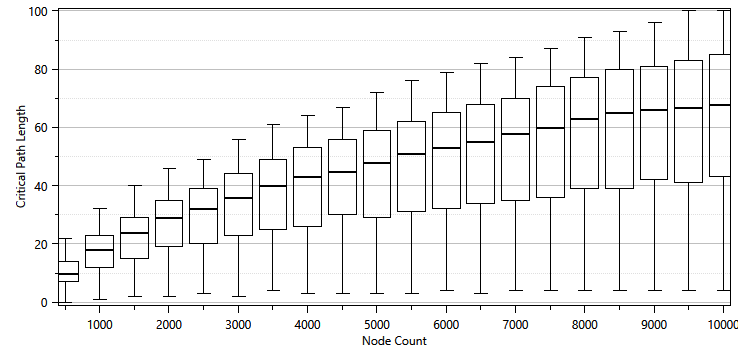
\includegraphics[width=0.9\textwidth]{figures/plots/boxplotnl.png}
	\caption{NodeCount to CriticalPathLength}
	\label{fig:scatterplotnl}
\end{figure}

As our plots get denser as we increase the node count linearly (Figure~\ref{fig:boxplotndelta}), we studied the relation between $\Delta$ and $l$ and got the expected result, a slightly similar curve as seen when comparing $n$ and $l$ (Figure~\ref{subfig:boxplotaveragedeltal}). Additionally, we plotted the same plot with a reduced data set (Figure~\ref{subfig:boxplotaveragedeltal8k}); we only looked at data that had a node count of $8,000$ and higher. This dataset produced the same curve when comparing $\Delta$ to $l$ without that restriction.

\begin{figure}[ht]
	\centering
	
\subcaptionbox{Complete dataset\label{subfig:boxplotaveragedeltal}}[.9\linewidth]
{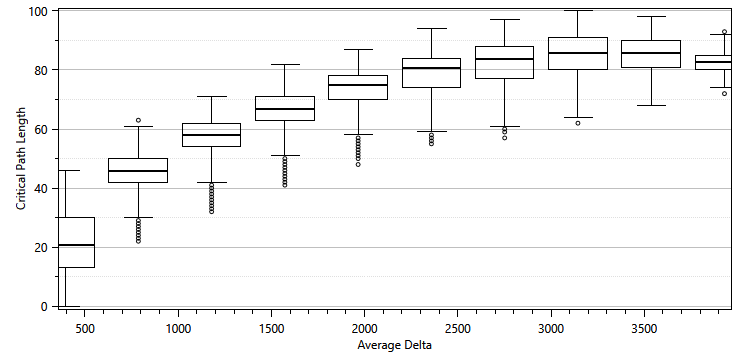
\includegraphics[width=.9\linewidth]{figures/plots/boxplotaveragedeltal.png}}

\end{figure}
\begin{figure}
\ContinuedFloat
\subcaptionbox{Only NodeCount > $8,000$\label{subfig:boxplotaveragedeltal8k}}[.9\linewidth]
{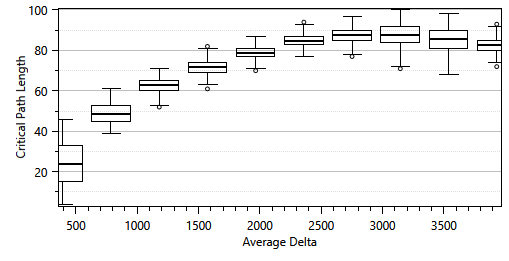
\includegraphics[width=.9\linewidth]{figures/plots/boxplotaveragedeltal8k.png}}

	\caption{Boxplots of the average in-degree compared to $l$}
	\label{fig:boxplotaveragedeltal}
\end{figure}

We observe that with increasingly high $\Delta$, $l$ actually decreases in length. Next, we compared $l$ to the difference in transmission ranges; as we expect, as the difference in transmission ranges in one graph gets bigger, so does $l$. However, as in the previous observation, we again have a decrease in $l$ as the range gets increasingly large. If we calculate $MaxRange/MinRange$ instead of $MaxRange-MinRange$, our plot still behaves similar.


\begin{figure}[ht]
	\centering
		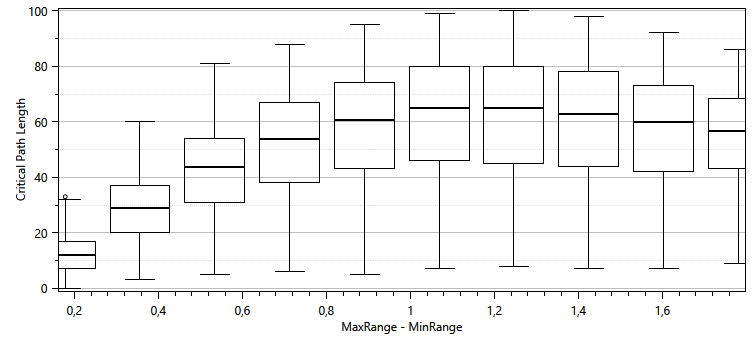
\includegraphics[width=0.9\textwidth]{figures/plots/boxplotrangediffl.png}
	\caption{Range difference compared to CriticalPathLength}
	\label{fig:scatterplotrangediffl}
\end{figure}

When looking at Plot~\ref{fig:boxplotstronglyconnectedcomponentsl}, comparing the strongly connected components of a graph with its $l$-value, we find that they seem to be related linearly, but when the number of strongly connected components reaches a certain tipping point, the $l$-value plummets rapidly and stays at a constant level.

\begin{figure}[ht]
	\centering
		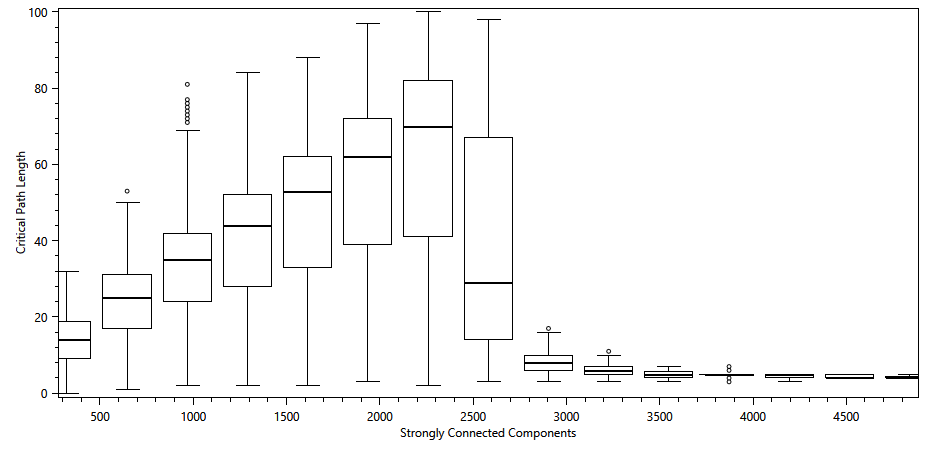
\includegraphics[width=0.9\textwidth]{figures/plots/boxplotstronglyconnectedcomponentsl.png}
	\caption{Strongly connected components in relation to $l$.}
	\label{fig:boxplotstronglyconnectedcomponentsl}
\end{figure}

\begin{figure}[ht]
	\centering
		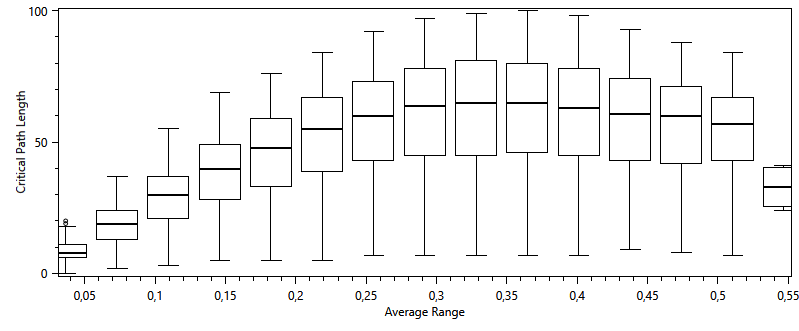
\includegraphics[width=0.9\textwidth]{figures/plots/boxplotaveragerangel.png}
	\caption{Average range in relation to $l$.}
	\label{fig:boxplotaveragerangel}
\end{figure}

The last plot we will show is Plot~\ref{fig:boxplotaveragerangel}, putting the average transmission range of nodes in relation to $l$. We observe the same curve that could be see on the other graphs, yet more clearly.


\newpage
\section{Discussion}

In this section we interpret the observations we made in the earlier section and discuss their implications.


Obviously, it was to be expected that when increasing the number of nodes on the same space, the average node-degree increases linearly. We can also exclude $n$ as a factor that defines $l$ as the Figure~\ref{subfig:boxplotaveragedeltal8k} shows that for a fixed $n$, the plot comparing $\Delta$ and $l$ looks exactly the same and in our setting, $\Delta$ is bound to grow linearly with network size.

From this we might assume that $l$ grows with roughly logarithmically with $\Delta$, which implies that as graphs get denser, the probability of a unidirectional chain forming gets bigger. We look at Figure~\ref{fig:boxplotstronglyconnectedcomponentsl} though, which gives us a very interesting observation. Because if a graph is more dense, this implies less strongly connected components, but we can clearly see that for a while, more strongly connected components lead to higher values of $l$. At some point, the value for $l$ drops dramatically, though, at which point the nodes are clustered into such a huge amount of small components that it is impossible for any huge structure to form.

So we interpret that a higher density does not ultimately form a higher value for $l$. In fact, if we look close at Figure~\ref{subfig:boxplotaveragedeltal}, we can see that $l$ begins to drop for huge values of $\Delta$. We can see the same behaviour when we compare the range difference of a graph to $l$ (Figure~\ref{fig:scatterplotrangediffl}). We get the biggest values for $l$ when the range-difference is approximately at $1$. This implies that there are nodes which link with almost every node in the graph down to nodes which are very local. By the way we give each node a random range withing a graphs range constraints, we can assert that the between the minimal range of a graph and the maximum range of a graph, the ranges of the nodes have an equal distribution. As the range difference of nodes surpasses $1$, more and more nodes can communicate with the whole graph, and they form a network of bidirectional communication links together (and any node which can reach them), which decreases the possibility of creating unidirectional communication links dramatically, yet increases $\Delta$ dramatically as well. And here is where we see the connection between the two values and also why $l$ decreases as $\Delta$ grows increasingly large.

The longest directed path in a communication graph with arbitrary transmission power is hence dependent on the standard deviation from the transmission ranges of all nodes (for a large enough number of nodes). This is no surprise, as with no deviation from the transmission ranges, we would have a uniform disk graph as a result, which by definition has no unidirectional communication link. The bigger the deviations from the average transmission range is, the bigger is the probability that one node $v$ could be placed just outside the range of another node $u$, with $v$ having a bigger range than $u$, creating a unidirectional communication link. Logically, as the probability for a single such link increases, the probability for many links forming a chain increases as well. This growth in $l$ is bounded, though, as transmission ranges themselves reach the size of the whole graph.

The last observation we shall state here is that for our more than $50,000$ simulations, $l$ was bounded at $100$. An interesting follow up study would be to increase the area of the simulation simultaneously with the node count, while leaving all other parameters intact, essentially increasing the nodecount without affecting $\Delta$, and observing whether higher values for $l$ will get generated that way.

The source-code for the simulator, the webservice and the plotting utility, as well as the test-data that was collected can be inspected and downloaded from GitHub\footnote{https://github.com/Manuel-S/graph-simulation}.



%% conclusion.tex
%%

%% ==================
\chapter{Conclusion}
\label{ch:conclusion}
%% ==================

In this paper we have shown that including unidirectional communication links in distributed algorithms is possible without much change to existing algorithms, yet they provide a new challenge for the algorithms themselves. For example, to get rid of a neighborhood search in the algorithms, we had to add $\Delta$ colors to the available color pool. In a way, we have shown that for randomized algorithm in directed graphs, the lack of a guarantee of neighbors respecting chosen colors leads to a bigger color pool. We present an algorithm which calculates a $\Delta+1$ coloring with an initialization in $O(\Delta+l\log n)$ and one algorithm which calculates a $2\Delta+1$ coloring without initialization in $O(l\log n)$.

We also show that the runtime of randomized algorithms depend on the factor $l$, which is the longest chain of unidirectional communication links in the graph, and observe that this value does in praxis play a definite role and is dependant on the variation in transmission ranges of nodes, as we generated test data using geometric calculations which represent the nature of the SINR model with variable transmission power.

We believe that distributed algorithms on directed graphs should be further evaluated as the fundamental problem of having no confirmation of message delivery is closely related to the physical SINR model with arbitrary transmission powers as well as generalizations of that using a signal decay model \cite{DBLP:journals/corr/BodlaenderH14}.

Further work can be done to decrease the amount of colors in Algorithm~\ref{alg:r2d+1}, for example by looking into the proof of Johansson \cite{johansson1999simple} that Luby's algorithm also works without the coin toss to produce a $\Delta+1$ coloring in $O(\log n)$ rounds, and to remove the necessity of nodes knowing the global degree $\Delta$ and accomodating for asynchronous wake up times.



%% --------------------
%% |   Bibliography   |
%% --------------------

\cleardoublepage
\phantomsection
\addcontentsline{toc}{chapter}{\bibname}

\iflanguage{english}
{\bibliographystyle{alpha}}
{\bibliographystyle{babalpha-fl}} % german style
\bibliography{references,abbrv}


%% ----------------
%% |   Appendix   |
%% ----------------

\cleardoublepage
%% appendix.tex
%%

%% ==============================
%\chapter{Appendix}
%\label{ch:Appendix}
%% ==============================
%\renewcommand\thefigure{\thechapter.\arabic{figure}}
\appendix

%\iflanguage{english}
{\addchap{Appendix}}	% english style
%{\addchap{Anhang}}	% german style

\section{Graphs}\label{appendix:graphs}

\begin{figure}[ht]
	\centering
		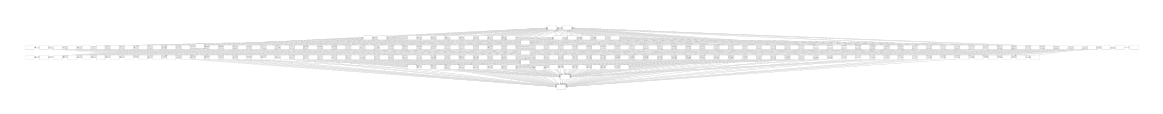
\includegraphics[width=0.90\textwidth]{figures/graphs/graphextrem.png}
	\caption{An example graph containing only $186$ nodes has over $9000$ edges.}
	\label{fig:graphextreme}
\end{figure}
\begin{figure}[ht]
	\centering
		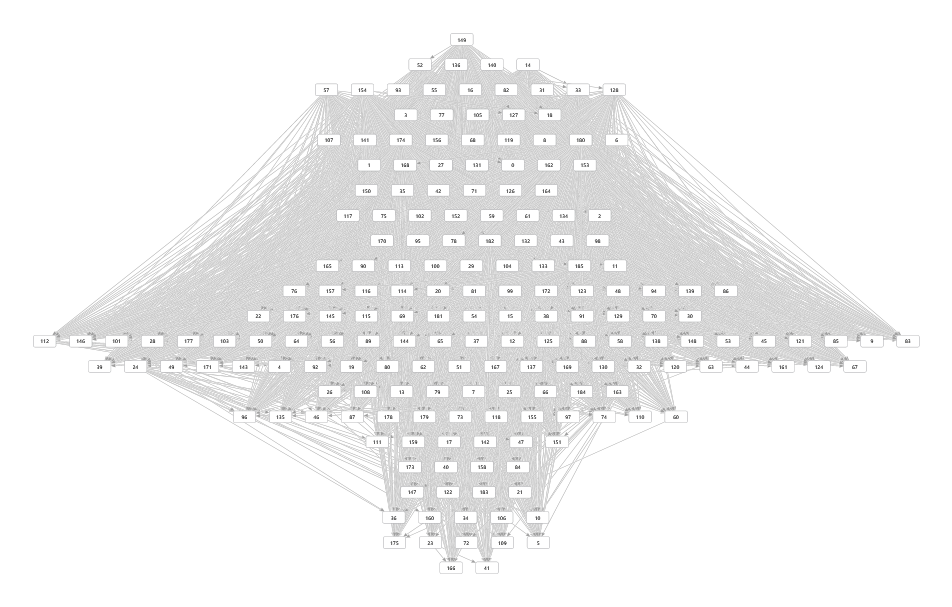
\includegraphics[width=0.90\textwidth]{figures/graphs/graphn186l22.png}
	\caption{The example graph's reduced version, which only contains unidirectional communication links. $l = 22$ can be efficiently computed in this subgraph. ($6310$ edges remain in this graph)}
	\label{fig:graphbetter}
\end{figure}
\newpage
\section{Plots}

\begin{figure}[ht]
	\centering
		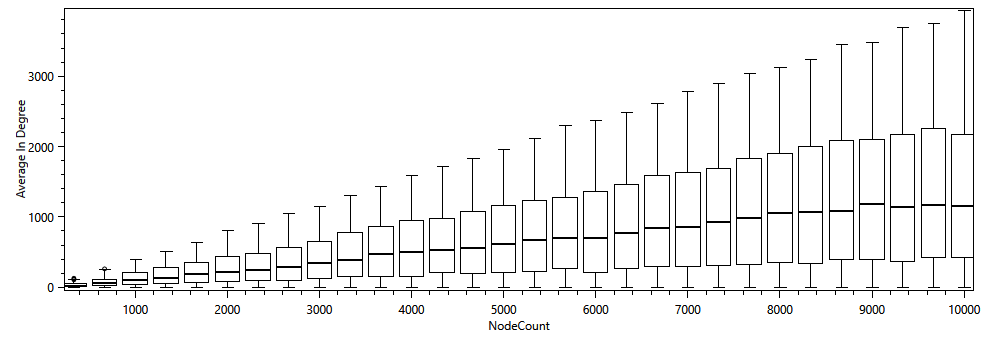
\includegraphics[width=0.90\textwidth]{figures/plots/boxplotndelta.png}
	\caption{Confirmation that $\Delta$ grows linearly with $n$ in our setting.}
	\label{fig:boxplotndelta}
\end{figure}

\begin{figure}[ht]
	\centering
		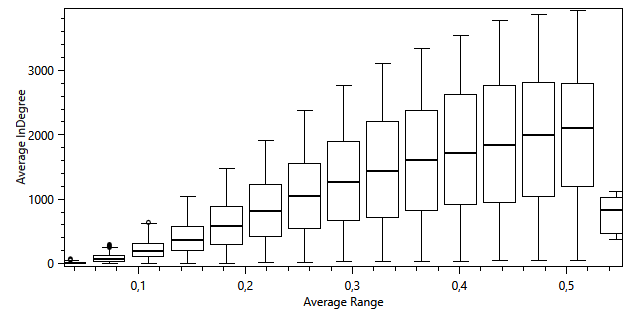
\includegraphics[width=0.90\textwidth]{figures/plots/boxplotaveragerangedelta.png}
	\caption{This plot shows that with an increase in transmission ranges, $\Delta$ increases proportionally.}
	\label{fig:boxplotaveragerangedelta}
\end{figure}






\end{document}
